\documentclass{article}

\usepackage{fancyhdr}
\usepackage{extramarks}
\usepackage{bm}
\usepackage{amsmath}
\usepackage{amsthm}
\usepackage{derivative}
\usepackage{amsfonts}
\usepackage{tikz}
\usepackage[plain]{algorithm}
\usepackage{algpseudocode}
\usepackage{graphicx}
\usepackage{tcolorbox}
\usepackage{esvect}
\graphicspath{ {tools/images/} }

\usetikzlibrary{automata, positioning}

%
% Basic Document Settings
%

\topmargin=-0.45in
\evensidemargin=0in
\oddsidemargin=0in
\textwidth=6.5in
\textheight=9.0in
\headsep=0.25in

\linespread{1.1}

\pagestyle{fancy}
\lhead{\hmwkAuthorName}
\chead{\hmwkClass \ \ \hmwkTitle}
\rhead{\firstxmark}
\lfoot{\lastxmark}
\cfoot{\thepage}

\renewcommand{\headrulewidth}{0.4pt}
\renewcommand{\footrulewidth}{0.4pt}

\setlength{\parindent}{0pt}

%
% Create Problem Sections
%

\newcommand{\enterProblemHeader}[1]{ \nobreak\extramarks{}{Problem \arabic{#1} continued on next page\ldots}\nobreak{}
\nobreak\extramarks{Problem \arabic{#1} (continued)}{Problem \arabic{#1} continued on next page\ldots}\nobreak{}
}

\newcommand{\exitProblemHeader}[1]{ \nobreak\extramarks{Problem \arabic{#1} (continued)}{Problem \arabic{#1} continued on next page\ldots}\nobreak{}
\stepcounter{#1}
\nobreak\extramarks{Problem \arabic{#1}}{}\nobreak{} }

\setcounter{secnumdepth}{0}

%
% Homework Problem Environment
%
% This environment takes an optional argument. When given, it will adjust the
% problem counter. This is useful for when the problems given for your
% assignment aren't sequential. See the last 3 problems of this template for an
% example.
%
\newenvironment{homeworkProblem}[1][-1]{ \ifnum#1>0
\setcounter{homeworkProblemCounter}{#1}
\fi
\subsection{Problem \arabic{homeworkProblemCounter}}
\setcounter{partCounter}{1}
\enterProblemHeader{homeworkProblemCounter} }{ \exitProblemHeader{homeworkProblemCounter}
}

%
% Homework Details
%   - Title
%   - Due date
%   - Class
%   - Section/Time
%   - Instructor
%   - Author
%

\newcommand{\hmwkTitle}{Notes}
\newcommand{\hmwkDueDate}{Spring 2024}
\newcommand{\hmwkClass}{Math 241}
\newcommand{\hmwkClassTime}{}
\newcommand{\hmwkClassInstructor}{}
\newcommand{\hmwkAuthorName}{\textbf{Terry Qiu}}

%
% Title Page
%

\title{
\vspace{2in}
\textmd{\textbf{\hmwkClass:\ \hmwkTitle}}\\ \normalsize
\vspace{0.1in}
\small{\hmwkDueDate}\\
\vspace{0.1in}
\large{\textit{\hmwkClassInstructor\ \hmwkClassTime}}
\vspace{3in}
}

\author{\hmwkAuthorName}
\date{}

\renewcommand{\part}[1]{\textbf{\large Part \Alph{partCounter}}
\stepcounter{partCounter}
\\}

%
% Various Helper Commands
%

% Useful for algorithms
\newcommand{\alg}[1]{\textsc{\bfseries \footnotesize #1}}

% For derivatives
\newcommand{\deriv}[1]{\frac{\mathrm{d}}{\mathrm{d}x} (#1)}

% For partial derivatives
\newcommand{\pderiv}[2]{\frac{\partial}{\partial #1} (#2)}

% Integral dx
\newcommand{\dx}{\mathrm{d}x}

% Alias for the Solution section header
\newcommand{\solution}{\textbf{\large Solution}}

% Probability commands: Expectation, Variance, Covariance, Bias
\newcommand{\E}{\mathrm{E}}
\newcommand{\Var}{\mathrm{Var}}
\newcommand{\Cov}{\mathrm{Cov}}
\newcommand{\Bias}{\mathrm{Bias}}

\begin{document}
	\newtcolorbox{mybox}[1] {colback=red!5!white,colframe=red!75!black,fonttitle=\bfseries,title=#1}

	\maketitle
	\newpage
	\tableofcontents
	\pagebreak
	\section{Vectors and the Geometry of Space}
	\subsection{12.4 Cross Product}
	The cross product of two vectors expresses a vector that is perpendicular to
	both the vectors.
	\begin{mybox}
		{Cross product} The cross product of two vectors $\vec{a}$ and $\vec{b}$ is given
		by

		\[
			\vec{a}\times \vec{b}= \langle a_{2}b_{3}-a_{3}b_{2},a_{3}b_{1}-a_{1}b_{3},
			a_{1}b_{2}-a_{2}b_{1} \rangle
		\]

		Notice also that the cross product of $\vec{a}$ and $\vec{b}$ can also be given
		by the determinant of the matrix
		\[
			\begin{vmatrix}
				\vec{i} & \vec{j} & \vec{k} \\
				a_{1}   & a_{2}   & a_{3}   \\
				b_{1}   & b_{2}   & b_{3}
			\end{vmatrix}
		\]
	\end{mybox}

	In other words, \\
	\[
		\vec{a}\times \vec{b}=
		\begin{vmatrix}
			a_{2} & b_{3} \\
			b_{1} & b_{3}
		\end{vmatrix}
		\vec{i}-
		\begin{vmatrix}
			a_{1} & a_{3} \\
			b_{2} & b_{3}
		\end{vmatrix}
		\vec{j}+
		\begin{vmatrix}
			a_{1} & a_{2} \\
			b_{1} & b_{2}
		\end{vmatrix}
		\vec{k}
	\]
	\\
	\begin{mybox}
		{Length of the cross product} If $\theta$ is the angle between $\vec{a}$ and
		$\vec{b}$ where $0 < \theta < \pi$ then the length of the cross product of vectors
		$\vec{a}$ and $\vec{b}$ is given by
		\[
			|\vec{a}\times \vec{b}| = |\vec{a}||\vec{b}|\sin(\theta)
		\]
	\end{mybox}
	The length of the cross product of $\vec{a}$ and $\vec{b}$ is also the area of
	the parallelogram composed by $\vec{a}$ and $\vec{b}$,
	\[
		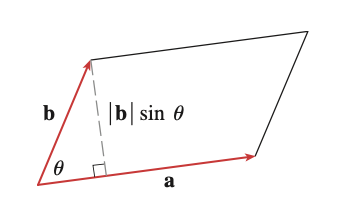
\includegraphics[scale=0.7]{Geo}
	\]
	\\ Note also that $\vec{a}$ and $\vec{b}$ are parallel only if, \\
	\[
		\vec{a}\times \vec{b}= 0
	\]
	\\ The volume of the parallelepiped determined by the vectors $\vec{a}$,
	$\vec{b}$ and $\vec{c}$ is given by what is known as the scalar triple product.
	\\

	\[
		V = |\vec{a}\cdot (\vec{b}\times \vec{c})|
	\]
	\[
		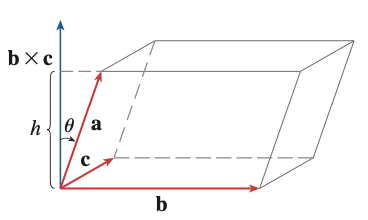
\includegraphics[scale=0.6]{TripleProduct}
	\]
	Notice that $|\vec{b}\times \vec{c}|$ is equal to the base area, and $|a|\cos(\theta
	)$ gives the height so V =$|\vec{b}\times \vec{c}||a|\cos(\theta) = \vec{a}\cdot
	(\vec{b}\times \vec{c})$. We need to apply the absolute sign to $\cos(\theta)$
	because it is possible that $\theta > \frac{\pi}{2}$

	\subsection{12.5 Equations of lines and vectors}

	The position vectors of all points on a line can be traced out by a vector equation
	determined by a known point on a line and a direction vector parallel to the direction
	of the line. Mathematically this means, \\
	\[
		\vec{r}= \vec{r_0}+ t\vec{v}
	\]
	\\ where $\vec{r}, \vec{r_0}, t, \text{and}$ $\vec{v}$ are the position vector
	of any point on the line, the position vector of a known point on the line, a scalar
	that can be any real number, and the direction vector that is parallel to the
	line, respectively. We can also write $\vec{r}$ with its components,
	\[
		\langle x,y,z \rangle =\langle x_{0}+ta,y_{0}+tb,z_{0}+tc \rangle
	\]
	Therefore, \\
	\[
		x=x_{0}+ta \ \ \ y=y_{0}+tb \ \ \ z=z_{0}+tc
	\]
	\\ This is known as a parametric equation of a line. Since the variables are given
	in terms of the variable $t$, it is possible to eliminate the vector $t$ by \\
	\[
		\frac{x-x_{0}}{a}= \frac{y-y_{0}}{b}= \frac{z-z_{0}}{c}
	\]
	\\ This is known as the symmetric or cartesian equation of a line. Notice that
	if the line passes through two points with position vectors $\vec{P_0}= \langle
	x_{0},y_{0},z_{0} \rangle$ and $\vec{P_1}= \langle x_{1},y_{1},z_{1} \rangle$,
	then we have \\
	\[
		\frac{x-x_{0}}{x_{1}-x_{0}}= \frac{y-y_{0}}{y_{1}-y_{0}}= \frac{z-z_{0}}{z_{1}-z_{0}}
	\]
	\\ since the direction vector is given by \\
	\[
		\vec{d}=
		\begin{pmatrix}
			a \\
			b \\
			c
		\end{pmatrix}
		=
		\begin{pmatrix}
			x_{1}-x_{0} \\
			y_{1}-y_{0} \\
			z_{1}-z_{0}
		\end{pmatrix}
	\]
	\\ If we wanted to find a line segment of a line and not the entire line, we can
	put the line into its vector equation with $t$ bounded by 0 and 1 inclusive,
	and with endpoints having the position vectors
	$\vec{P_0}= \langle x_{0},y_{0},z_{0} \rangle$ \text{and}
	$\vec{P_1}= \langle x_{1},y_{1},z_{1} \rangle$ \\
	\[
		\vec{r}= \vec{r_0}+ (\vec{r_1}-\vec{r_0})t
	\]
	Realise that this makes
	$\vec{r}= \vec{r_0}\text{ when }t = 0 \text{ and }\vec{r}= \vec{r_1}\text{ when
	}t = 1$
	\\ \\
	\begin{mybox}
		{Equation of a plane} The equation of a plane is defined with respect to a vector
		orthogonal to the point and an known point on the plane. Given an arbitrary
		point on the plane with position vector $\vec{r}= \langle x,y,z \rangle$, a known
		point with position vector $\vec{r_0}= \langle x_{0},y_{0},z_{0} \rangle$,
		and a normal vector $\vec{n}= \langle a,b,c \rangle$ we have
		\[
			\vec{n}\cdot (\vec{r}-\vec{r_0}) = 0
		\]
		So an equation of a plane through
		$\vec{r_0}= \langle x_{0},y_{0},z_{0} \rangle$ with
		$\vec{n}= \langle a,b,c \rangle$ is
		\[
			a(x-x_{0})+b(y-y_{0})+c(z-z_{0}) = 0
		\]
	\end{mybox}
	We can find the $x,y,z$ intercepts by setting the two variables other from the
	one we are trying to find as 0. Two find the angle between two planes we can
	use the equation
	\[
		\cos{\theta}= \frac{\vec{n_1} \cdot \vec{n_2} }{|\vec{n_1}||\vec{n_2}|}
	\]
	where $\vec{n_1}$ and $\vec{n_2}$ are the normal vectors of the plane. \\ \\ If
	we are asked to find the equation of the line of intersection of the plane we can
	find the cross product of the normal vectors of the two planes which will yield
	a direction vector that is perpendicular to both the normal vectors. In other
	words, we will get a direction vector that is parallel to both planes and a valid
	direction vector to form the vector equation of the line. For example, given the
	equations $x+y+z =1$ and $x-2y+3z=1$, the direction vector of the line will be
	given by
	\[
		\begin{vmatrix}
			i & j  & k \\
			1 & 1  & 1 \\
			1 & -2 & 3
		\end{vmatrix}
		= 5\vec{i}- 2\vec{j}- 3\vec{k}
	\]

	Then we can find a point on the line by setting one variable as $0$. This
	choice of variable is dependent on which plane the line will intersect, and there
	will always be one plane that the line will intersect. In this case we notice
	that the line is not parallel with the $xy$ plane, so the line will intersect the
	$xy$ plane once. Therefore we can let $z=0$ which give us the equations
	\[
		x+y=1 \text{ and }x-2y=1
	\]
	solving this system of equation will yield the point $(1,0,0)$. Why does solving
	the plane gives us a point on the line? After all the intersection of the two
	planes will have a line of intersection with the planes of the graph. However,
	notice that solving a system of equations involving the \textbf{two} equations
	of the plane implies that the answer will be a point on the line, because the
	answer will be one that is on both the equations. \\ \\
	\begin{mybox}
		{Distance from point to plane} The distance D from the point $P_{1}(x_{1},y_{1}
		,z_{1})$ to the plane $ax+by+cz+d=0$ is
		\[
			D=\frac{|ax_{1}+by_{1}+cz_{1}+d|}{\sqrt{a^{2}+b^{2}+c^{2}}}
		\]
		We can apply this to two skew lines by taking any point on one line as $P_{1}$
		and the plane as the plane the other line is on.
	\end{mybox}
	\subsection{12.6 Cylinders and Quadric Surfaces}
	Cylinders are surfaces that consist of all lines(\textbf{rulings}) that are parallel
	to a given line and pass through a given plane curve. $z=x^{2}$ is such a
	cylinder and its rulings are parallel to the $y$-axis.
	\[
		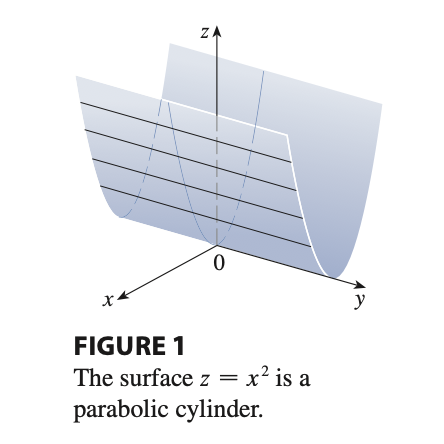
\includegraphics[scale=0.9]{Cylinder}
	\]
	If one of the variables $x$, $y$, and $z$ is missing from the equation, then
	the surface is a cylinder and its rulings are parallel to the missing variable.

	Traces are the cross sections of a curve, and the traces that is parallel to a
	given plane can be found by setting a variable as a constant $k$. For example,
	suppose that we have the quadric surface defined by the equation

	\[
		x^{2}+\frac{y^{2}}{9}+\frac{z^{2}}{4}= 1
	\]

	To find the trace of the graph that is parallel to the $xy-$ plane, we could
	set the variable $z$ to $0$. In general, the trace of a quadric surface can be
	found by setting a particular variable to $k$ depending on the plane which we
	want our traces to be parallel to. In the case of the function that we just saw,
	the horizontal trace in the plane $z=k$ is

	\[
		x^{2}+\frac{y^{2}}{9}+\frac{k^{2}}{4}= 1
	\]
	\pagebreak
	\section{Vector Functions}
	\subsection{13.1 Vector valued functions and space curves}

	A vector valued function is a function that takes in a real number and outputs
	a vector. If we are interested in vector functions of three dimensions, the
	components of vector functions in three dimensiosn are also functions.

	\[
		\vec{r}(t) = \langle f(t), g(t), h(t)\rangle = f(t)\vec{i}+g(t)\vec{j}+h(t)\vec
		{k}
	\]
	The limit of a vector function $\vec{r}(t)$ is

	\[
		\lim_{x \to a}\vec{r}(t) = \langle \lim_{x \to a}f(t), \lim_{x \to a}g(t), \lim
		_{x \to a}h(t) \rangle
	\]

	A vector function is \textbf{continuous at a} if

	\[
		\lim_{t \to a}\vec{r}(t) = \vec{r}(a)
	\]

	\textbf{Space curves are the set of all points traced out by the tip of a
	vector function.}

	\subsection{13.2 Derivatives and Integrals of Vector Functions}
	\begin{mybox}
		{Derivative of a vector function} The derivative of a vector function is defined
		similarly to the derivative to a regular function. In fact

		\[
			\frac{d\vec{r}}{dt}= \vec{r}\,'(x)=\lim_{h \to 0}\frac{\vec{r}\,(t+h)-\vec{r}\,(t)}{h}
		\]

		Furthermore

		\[
			\vec{r}\,'(t) = \langle f'(t), g'(t), h'(t)\rangle = f'(t)\vec{i}+g'(t)\vec
			{j}+h(t)\vec{k}
		\]
	\end{mybox}
	$\vec{r}\,'(t)$ gives the tangent vector of the point at some point $p$ and the
	tangent line at point $p$ is defined to be the line that is parallel to the tangent
	vector through $p$. The unit tangent vector is the tangent vector multiplied
	by the reciprocal of the magnitude of itself just like finding the unit vector
	in the direction of any other vector \\ \\
	\[
		\vec{T(t)}=\frac{\vec{r}\,'(t)}{|\vec{r}\,'(t)|}
	\]
	\\ \\ If $\vec{r}(t) = c$, then $\vec{r}\,'(t)$ is orthogonal $\vec{r}(t)$ for
	all $t$.
	\newpage
	The definite integral is defined in approximately the same way
	\[
		\int_{a}^{b}\vec{r}(t)\, dt = \left( \int_{a}^{b}f(t)\, dt \right) \vec{i}+ \left
		(\int_{a}^{b}\vec{g}(t)\, dt\right)\vec{j}+ \left(\int_{a}^{b}\vec{r}(t)\, dt
		\right)\vec{k}
	\]
	\\ \\ FTC could also be applied in the same way for a vector function, in fact
	\[
		\int_{a}^{b}\vec{r}(t)\, dt = \left[ \vec{R}(t) \right]_{a}^{b} = \vec{R}(b)
		- \vec{R}(a)
	\]
	\subsection{13.3 Arc Length and Curvature}
	\begin{mybox}
		{Arc Length of a space curve} The arc length of a space curve is defined in a
		similar way as that of a plane curve. If we have the vector equation
		$\vec{r}(t) = \langle f(t), g(t), h(t)\rangle$ and $a \leq t \leq b$. If the
		curve is traversed only once from $a$ to $b$ then
		\[
			L = \int_{a}^{b}\sqrt{ [f'(t)]^{2} + [g'(t)]^{2} + [h'(t)]^{2}}\, dt
		\]
		which can be conveniently written as
		\[
			L = \, \int_{a}^{b}|\vec{r}\,'(t)|\, dt
		\]

		since

		\[
			|\vec{r}\,'(t)| = |\langle f'(t), g'(t), h'(t)\rangle| = \sqrt{ [f'(t)]^{2},
			[g'(t)]^{2}, [h'(t)]^{2}}
		\]
	\end{mybox}
	The arc length function is given by
	\[
		s(t) = \int_{a}^{t}\sqrt{\left(\frac{dx}{du}\right)^{2}+ \left(\frac{dy}{du}\right)^{2}
		+ \left(\frac{dz}{du}\right)^{2} }\, du
	\]
	It gives the length of the space curve from $a$ to $t$.

	The curvature of a curve is defined as
	\[
		\kappa = \frac{|d\vec{T}|}{ds}
	\]
	where $\vec{T}$ is the unit tangent vector. The curvature of a curve is the
	magnitude of the rate of change of the unit tangent vector with respect to arc
	length. The curvature of a somewhere can also be expressed as
	\[
		\kappa(t) = \frac{|\vec{T}\,'(t)|}{|\vec{r}\,'(t)|}
	\]
	and also
	\[
		\kappa(t) = \frac{|\vec{r}\,'(t)\times \vec{r}\,''(t)|}{|\vec{r}\,'(t)|^{3}}
	\]
	moreover
	\[
		\kappa(x) = \frac{|f\,''(x)|}{[1+(f'(x))^{2}]^{2/3}}
	\]

	\section{Partial Derivatives}
	\subsection{14.1 Functions of several variables}

	If $f$ is a function of two variables with domain D, then the graph of $f$is the
	set of all points $(x,y,z)$ in $\mathbb{R}^{3}$ such that $z=f(x,y)$ and $(x,y)$
	is in $D$

	A level curve of a function $f$ are the curves with the equations $f(x,y) = k$
	, where $k$ is a constant. It would graph all the $x$ and $y$ values that satisfies
	the function $f$ when $z=k$ and project them onto the $x-y$ plane as is shown in
	the figure below.

	\[
		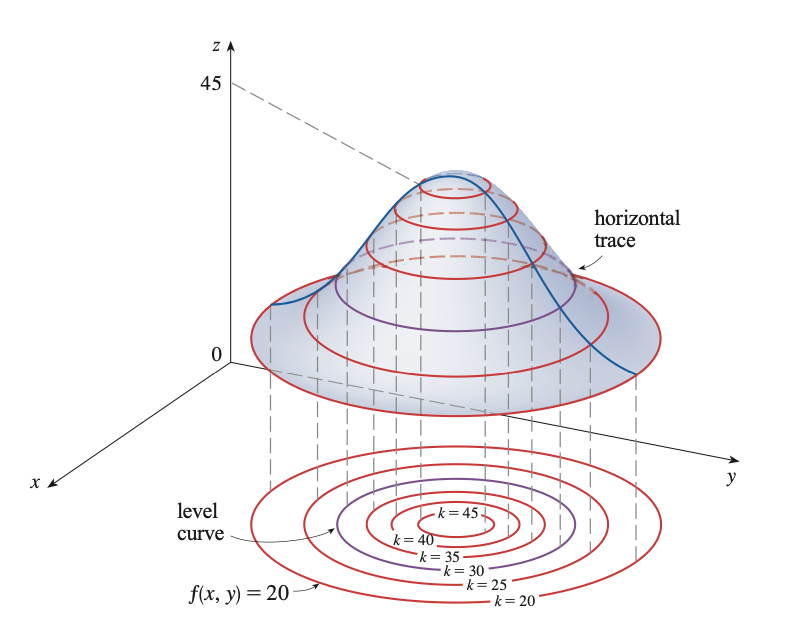
\includegraphics[scale=0.6]{LevelCurves}
	\]
	Functions of three variables behave similarly as that of functions of two variables.
	Functions of three variables are still rules that assigns the triplets
	$(x,y,z)$ that are elements of the set $\mathbb{R^3}$ to a unique real number
	denoted by $f(x,y,z)$. Its impossible to visualize the graphical representation
	of a function of three variables like that of functions of two variables. But
	it is possible to see that the \textbf{level surfaces} are the projections of the
	traces of the functions down to $\mathbb{R^3}$.

	For example, suppose we have a function of three variables defined by the
	equation $f(x,y,z) = x^{2}+y^{2}+z^{2}$. If we let $f(x,y,z) =k$ we see that the
	level surfaces form concentric spheres with radius $\sqrt{k}$.
	\[
		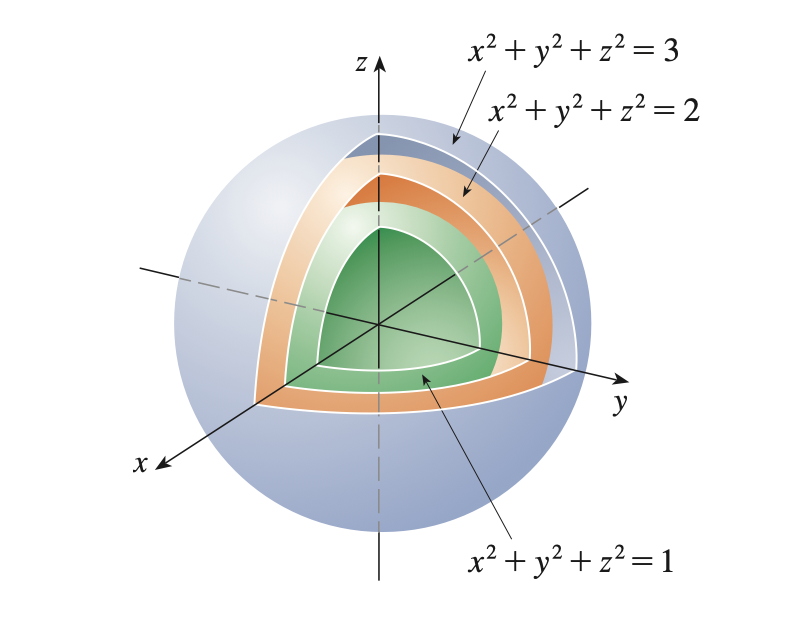
\includegraphics[scale=0.6]{FourD}
	\]

	Similar concepts useful in functions of two variables can be extended to functions
	of $n$ or more variables. A function of $n$ variables would be a rule that
	assigns a number $z=f(x_{1},x_{2},...,x_{n})$ to an $n$ tuple
	$(x_{1},x_{2},x_{3},...,x_{n})$ that is an element of $\mathbb{R}^{n}$.

	\subsection{14.2 Limits and Continuity}
	In general, we use the notation
	\[
		\lim_{(x,y) \to (a,b)}f(x,y) = L
	\]
	to indicate that the values of $f(x,y)$ approach some number L as the point $(x
	,y)$ approaches the point $(a,b)$. To show that a limit does not exist at some
	point $(a,b)$ for a function of two variables we can show that $(x,y)$
	approaches a different value for different paths. For example, if we are asked
	to show that the limit of
	\[
		\lim_{(x,y) \to (0,0)}\frac{x^{2}-y^{2}}{x^{2}+y^{2}}
	\]. We can show that we get different values when $(x,y)$ approaches $(0,0)$ along
	the $x$ axis and the $y$ axis. If $(x,y)$ approaches $(0,0)$ from the $y$ axis
	we have $f(0,y) = \frac{x^{2}}{x^{2}}= 1$, on the other hand if $(x,y)$ approaches
	$(0,0)$ from the $x$ axis we have $f(0,y) = \frac{-y^{2}}{y^{2}}= -1$. So we
	have demonstrated that the limit does not exist by showing that the value of
	the function at a given point is different when approached from different
	directions. \\ \\ When dealing with polynomial or rational functions of two variables
	we can compute the limit by direct substitution.
	\begin{mybox}
		{Continuity for functions of two variables} A function is continuous at a point
		$(a,b)$ if
		\[
			\lim_{(x,y) \to (a,b)}f(x,y) = f(a,b)
		\]
		in all the directions that $x,y$ can approach $a,b$
	\end{mybox}

	\subsection{14.3 Partial Derivatives}
	For a function $f$ of two variables, if we keep one variable fixed, say $y$,
	and let the other vary, say $x$, then we are really considering a function of
	one variable $g(x) = f(x,b)$ and if the function $g$ has a partial derivative
	at $a$, we call the derivative the partial derivative of $f$ at $a,b$.
	\begin{mybox}
		{Partial derivatives of functions of two variables} Formally, if $f$ is a
		function of two variables, its partial derivatives are the functions $f_{x}$
		and $f_{y}$ defined by
		\[
			f_{x}(x,y) = \lim_{h\to 0}\frac{f(x+h,y)-f(x,y)}{h}
		\]
		\[
			f_{y}(x,y) = \lim_{h\to 0}\frac{f(x,y+h)-f(x,yr)}{h}
		\]
	\end{mybox}
	$z=f(x,y)$ represents the surface $S$ and the graph of $f(x,y)$, if $f(a,b) =c$,
	then the point $P(a,b,c)$ is a point on the surface. If we fix the $y$ variable
	to be $b$ and vary only the $x$ variable, we would be finding the $x$ values
	such that it is on the vertical plane $y=b$, and is intersecting the surface,
	a similar thing can be said when we are fixing $x$ to a particular value. They
	form the traces of the surface in $y=b$ and in $x=a$ and they are represented by
	the figure below as $C_{1}$ and $C_{2}$ respectively. Notice that the curve
	$C_{1}$ is represented by the function $g(x) = f(x, b)$ and $C_{2}$ is
	represented by the function $G(y) = f(a,y)$. Consequently, we know that their
	slopes are given by the partial derivative with respect to $x$ at $(a,b)$ and
	the partial derivative of $y$ at $(a,b)$.
	\[
		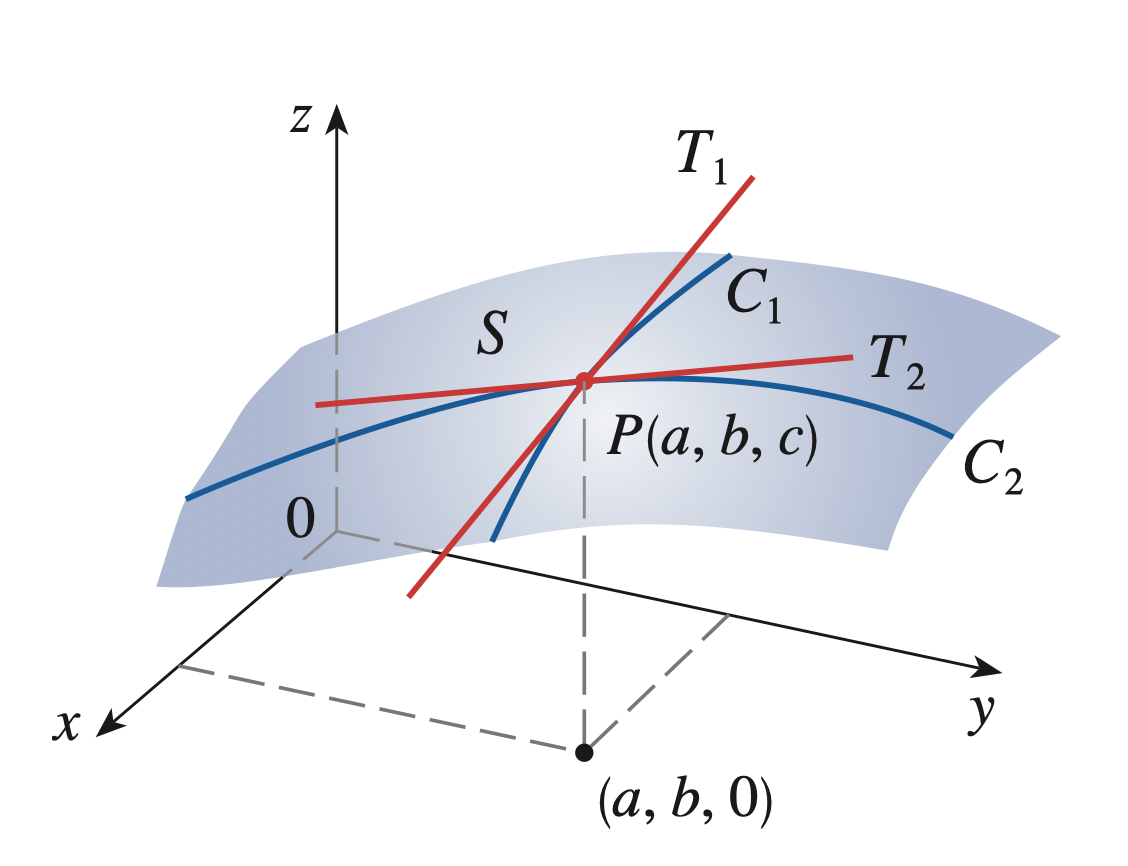
\includegraphics[scale=0.4]{PartialDerivatives}
	\]
	The partial derivative of functions of three or more variables could be defined
	in a similar fashion as it is defined for functions of two variables. They
	revolve around the same central idea of measuring the change of a particular
	variable when keeping one variable constant. \\ \\ $f_{xx}$ means the partial derivative
	of $f$ with respect to $x$ and then differentiated again with respect to $x$.
	In a similar logic, $f_{xy}$ would denote the partial derivative with respect $x$
	and then to $y$. \\ \\ Partial derivatives are incorporated in partial
	differential equations, which have important consequences in science and engineering.
	\textbf{Laplace's equation} after Pierre Laplace $(1749-1827)$, for example, play
	a role in problems such as heat conduction fluid flow, and electric potential.
	\[
		\pdv[order={2}]{u}{x}+ \pdv[order={2}]{u}{y}= 0
	\]

	\subsection{14.4 Tangent Planes and Linear Approximations}
	If we suppose that some surface $S$ has the equation $z=f(x,y)$, and let $P(x_{0}
	,y_{0},z_{0})$ be a point on $S$. Then again we have two curves $C_{1}$ and
	$C_{2}$ which are the traces of the curve in $y=y_{0}$ and $x=x_{0}$. If $T_{1}$
	and $T_{2}$ are tangent lines to the curve, then the \textbf{tangent plane} of
	the surface at $P$ will be the plane that contains both $T_{1}$ and $T_{2}$.\\\\

	\[
		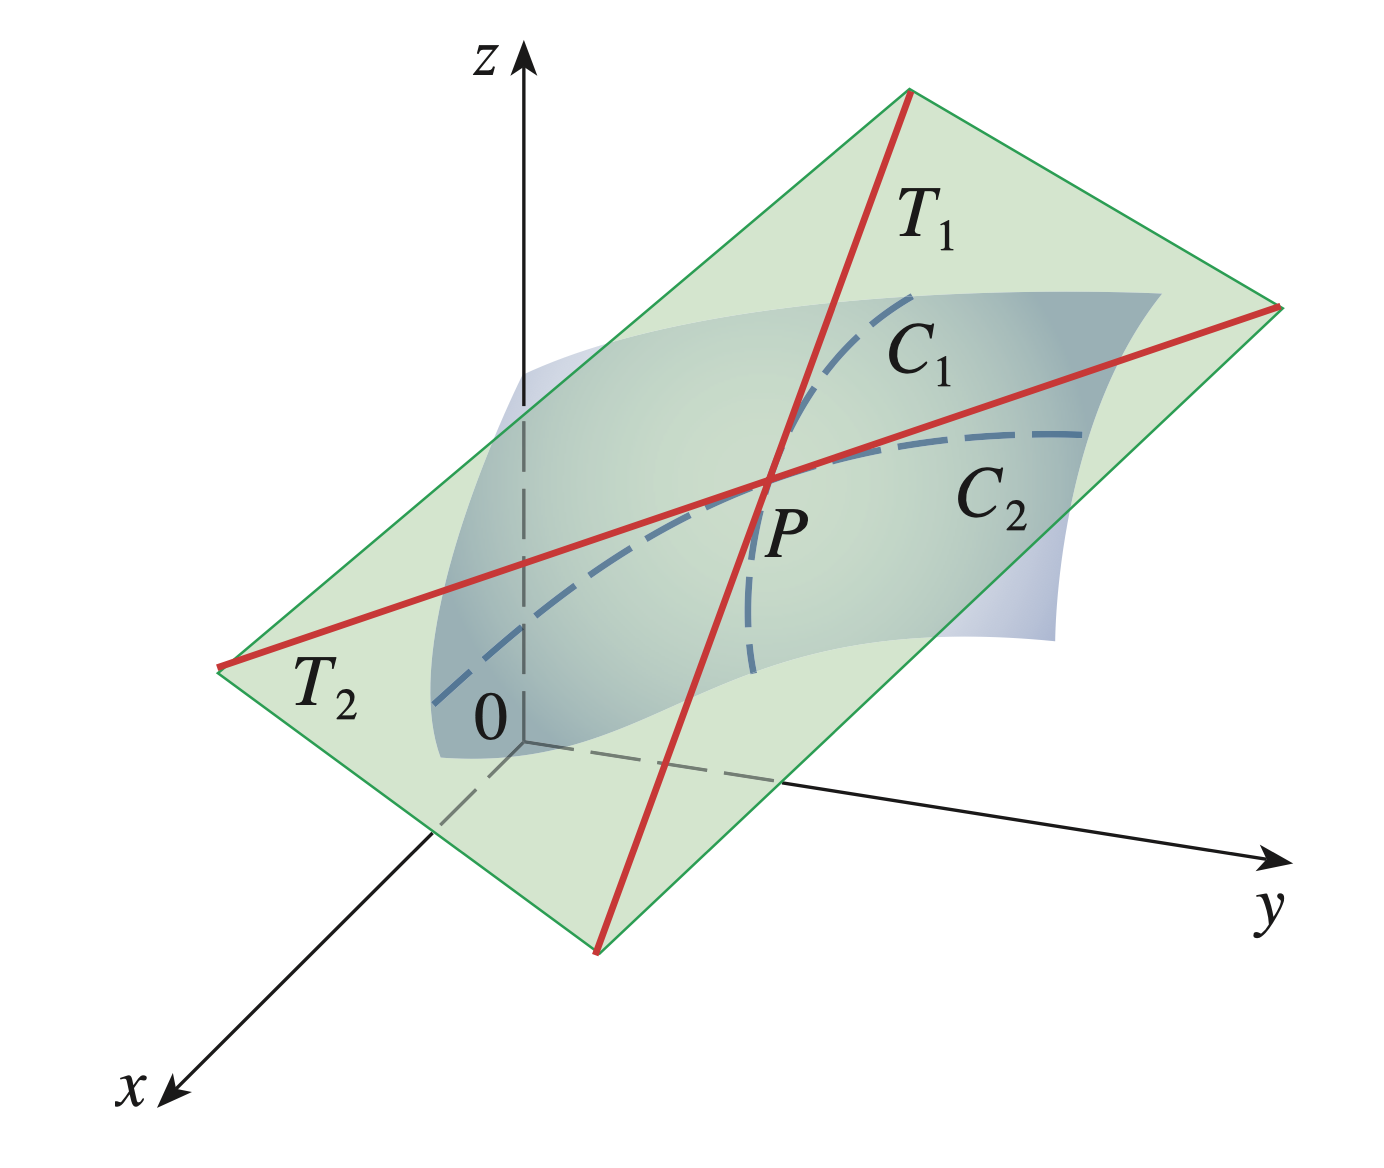
\includegraphics[scale=0.29]{TangentPlane}
	\]
	From the previous sections we know that the equation of any plane is defined by
	the equation $A(x-x_{0})+B(y-y_{0})+C(z-z_{)} = 0$, where $A,B$ and $C$ are
	$x,y,z$ components of the normal vector respectively. If we divide both sides by
	$C$, we have $z-z_{0} = -\frac{A}{C}(x-x_{0})-\frac{B}{C}(y-y_{0})$, let $a=-\frac{A}{C}$
	and $b= -\frac{B}{C}$, we have $z-z_{0} = -a(x-x_{0})-b(y-y_{0})$. The intersection
	of this plane with the plane $y=y_{0}$ will give us the equation of the tangent
	line $T_{1}$, so we must have $a=f_{x}(x_{0},y_{0})$, similarly we have $b=a=f_{y}
	(x_{0},y_{0})$
	\begin{mybox}
		{Equation of the tangent plane at some point} In fact an equation of the tangent
		plane to the surface $z=f(x,y)$ at the point $P(x_{0},y_{0},z_{0})$ is given
		by the equation
		\[
			z-z_{0} = f_{x}(x_{0},y_{0})(x-x_{0}) +f_{y}(x_{0},y_{0})(y-y_{0})
		\]
	\end{mybox}

	\begin{mybox}
		{Linear approximation} The linear approximation of $f(x,y)$ near some point is
		simply the linear function that describes the tangent plane. Notice that
		$f(a,b)$ is simply $z_{0}$, expressed as the image of $x$ and $y$.
		\[
			L(x,y) = f(a,b) + f_{x}(a,b)(x-a) + f_{y}(a,b)(y-b)
		\]
	\end{mybox}
	The total differential or the differential $dz$ is defined by the equation
	\[
		dz = f_{x}(x,y)dx+f_{y}(x,y)dy
	\]
	It gives us the change in the $z$ value of the tangent plane instead of the
	actual point. However, when $dx$ and $dy$ are small, $dz$ approximates the actual
	change in $z$ value well.
	\subsection{14.5 The Chain Rule}
	\begin{mybox}
		{The general case of the chain rule for partial} If the dependent variable $u$
		is a function of $n$ intermediate variables $x_{1},x_{2},...,x_{n}$, each of
		which is a function of $m$ independent variables $t_{1}, t_{2},..., t_{m}$. Then
		$u$ is a function of $t_{1}, t_{2},...,t_{m}$ and we have
		\[
			\pdv{u}{t_i}= \pdv{u}{x_1}\pdv{x_1}{t_i}+ \pdv{u}{x_2}\pdv{x_2}{t_i}+...+\pdv
			{u}{x_n}\pdv{x_n}{t_i}
		\]
	\end{mybox}
	Consider the example where we have a dependent variable $w= f(x,y,z,t)$ and
	the intermediate variables $x=x(u,v)$, $y=y(u,v)$, $z=z(u,v)$, and $t=t(u,v)$.
	Then,
	\[
		\pdv{w}{u}=\pdv{w}{x}\pdv{x}{u}+ \pdv{w}{y}\pdv{y}{u}+ \pdv{w}{z}\pdv{z}{u}+
		\pdv{w}{t}\pdv{t}{u}
	\]
	The partial derivative of $w$ with respect to $s$ could be obtained in a similar
	fashion. \\\\ If we suppose that the function $F(x,y)=0$ defines $y$ implicitly
	as a function of and if $y=f(x)$, then we can take the partial derivative of
	both sides and conduct algebraic manipulation to obtain a equation for the
	derivative of $y$ with respect to $x$. In fact\\
	\[
		\frac{dy}{dx}= -\frac{F_{x}}{F_{y}}
	\]

	\subsection{14.6 Directional Derivatives and the Gradient Vector}
	The directional derivative can give us the rate of change of a function of two
	or more variables in any direction. Suppose that we want to find the rate of
	change of $z$ at $(x_{0},y_{0})$ in the direction of some vector
	$\vec{u}= \langle a, b \rangle$. Consider the possibility that this point lies
	on the surface defined by $z=f(x,y)$ then we have $z_{0} = f(x_{0},y_{0})$. So
	$P(x_{0},y_{0},z_{0})$ lies on $S$. We would always be able to define a plane in
	the direction of $\vec{u}$ that contains the point $P$. Suppose there exist
	some other point $Q(x,y,z)$ on the curve of intersection between the surface
	and the plane. Then the projection onto the $x-y$ plane will be $P'(x_{0},y_{0}
	,0)$ and $Q'(x,y,0)$.

	\[
		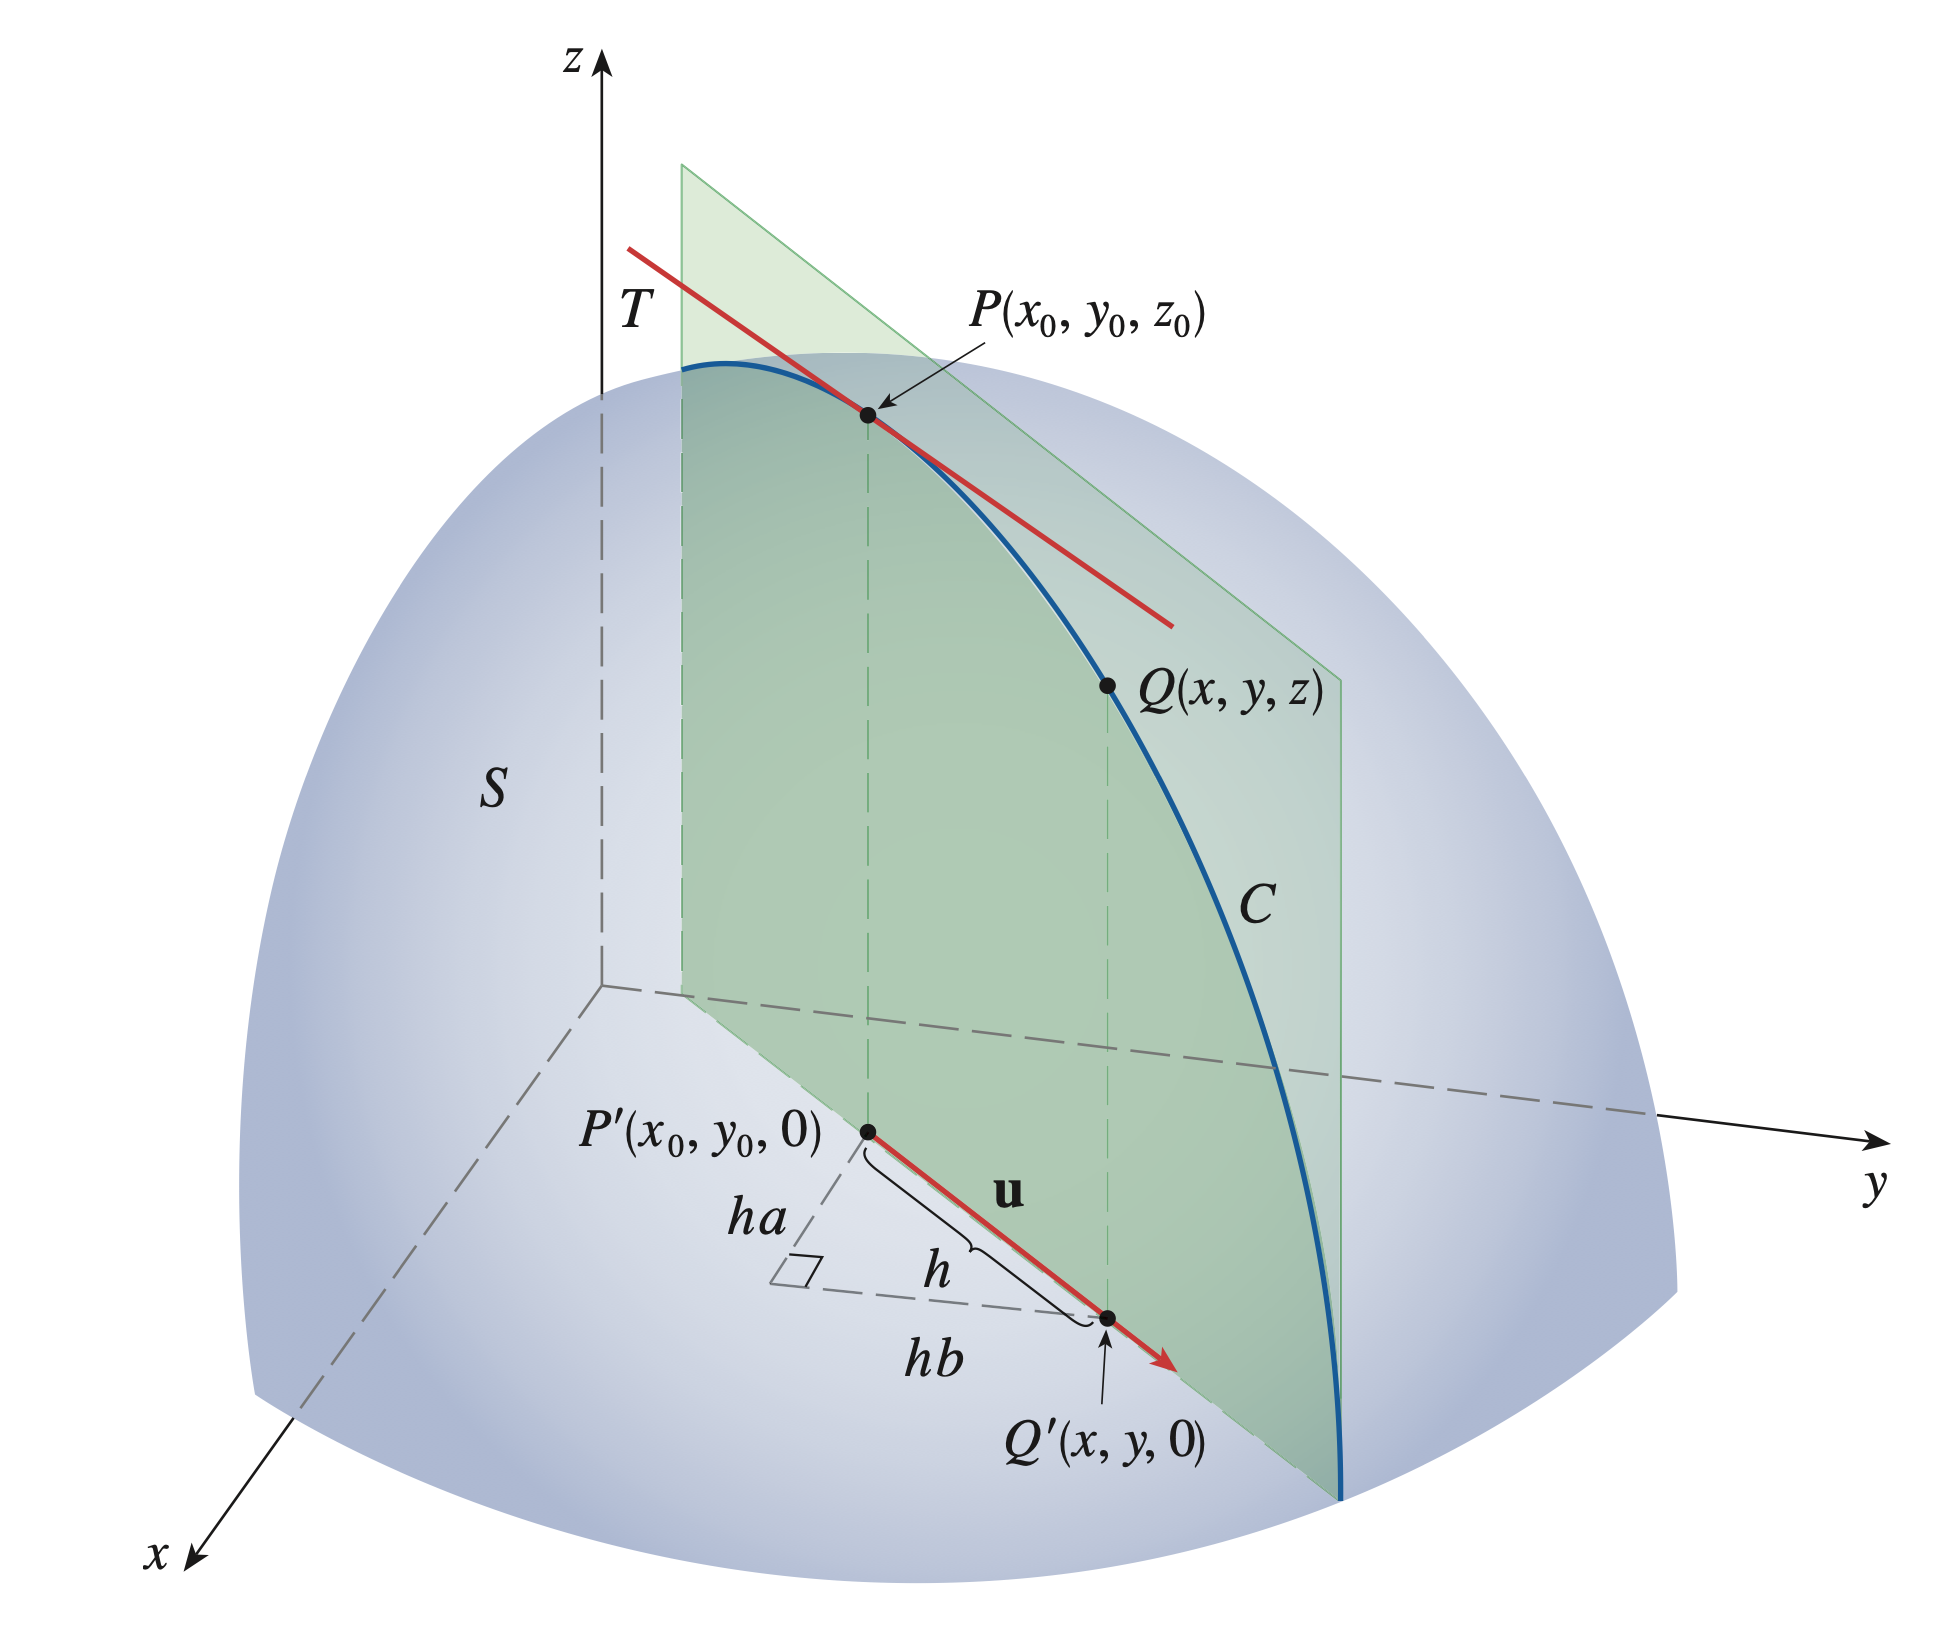
\includegraphics[scale=0.3]{DirectionalDeriv}
	\]

	Given any arbitrary two points on the plane, the line formed by their projection
	on the $xy$ will always be perpendicular to the normal vector. Realize that
	the unit vector $\vec{u}$ is also perpendicular to the normal vector. Hence the
	line conjoined by the two points must be parallel to the unit vector $\vec{u}$.
	Therefore, we have $\overrightarrow{P'Q'}= \langle ha, hb \rangle$, that
	$\overrightarrow{P'Q}$ can be expressed as the scalar multiple of the unit
	vector. Finally, $x=x_{0}+ha$ and $y=y_{0} +ha$. \\ \\ Now since, we can
	express $x,y$ in terms of the increment of known positions in the direction of
	some vector $\vec{u}= \langle a,b \rangle$, we have \\
	\[
		\frac{\Delta z}{h}= \frac{z-z_{0}}{h}= \frac{f(x_{0}+ha,y_{0} + hb) - f(x_{0},y_{0})}{h}
	\]
	\\ It is clear then that the directional vector of $f$ at $(x_{0},y_{0})$ in the
	direction of a unit vector $\vec{u}= \langle a,b \rangle$ \\
	\[
		D_{u}f(x_{0},y_{0}) = \lim_{h \to 0}\frac{f(x_{0}+ha,y_{0} + hb) - f(x_{0},y_{0})}{h}
	\]
	\\
	\begin{mybox}
		{Directional Derivatives} It is possible to prove the following equality for
		directional vectors
		\[
			D_{u}f(x,y) = f_{x}(x,y)a + f_{y}(x,y)b
		\]
		where $a,b$ are the components of the direction vector $\vec{u}= \langle a, b
		\rangle$
	\end{mybox}
	Notice that
	\begin{align*}
		D_{u}f(x,y) & = f_{x}(x,y)a + f_{y}(x,y)b                                       \\
		            & = \langle f_{x}(x,y),f_{y}(x,y) \rangle \cdot \langle a,b \rangle \\
		            & = \langle f_{x}(x,y),f_{y}(x,y) \rangle \cdot \vec{u}
	\end{align*}
	The first vector of this dot product is known as the gradient of $f$.
	\begin{mybox}
		{Gradient of a function of two variables} If $f$ is a function of two variables
		$x$ and $y$, then the gradient $f$ is the vector function $\nabla f$ defined
		by
		\[
			\nabla f(x,y) = \langle f_{x}(x,y), f_{y}(x,y) \rangle
		\]
		and the directional derivative in the direction of the unit vector $\vec{u}$
		\[
			D_{f}(x,y) = \nabla f(x,y) \cdot \vec{u}
		\]
	\end{mybox}

	We can naturally extend the definition of the directional derivative to the three
	dimensions. The directional derivative of some function $f$ at
	$(x_{0},y_{0},z_{0})$ in the direction of a unit vector
	$\vec{u}=\langle a,b,c \rangle$ is
	\[
		D_{u}f(x_{0},y_{0},z_{0}) = \lim_{h \to 0}\frac{f(x_{0} + ha, y_{0} + hb, z_{0}
		+ hc) - f(x_{0},y_{0},z_{0})}{h}
	\]
	if the limit exists. By a similar approach to functions of two variables we can
	show that
	\[
		\nabla f(x,y,z) = \langle f_{x}(x,y,z),f_{y}(x,y,z),f_{z}(x,y,z) \rangle
	\]
	and that
	\[
		D_{u} f(x,y,z) = \nabla f(x,y,z) \cdot \vec{u}
	\]
	\begin{mybox}
		{Maximization of directional derivative} Since $D_{u}f = \nabla f \cdot \vec{u}
		= |\nabla f||\vec{u}|\cos\theta$. $D_{u}f$ is maximized when $\theta = 0$, in
		other words, when we are trying to find the directional vector in the
		direction of the gradient of $f$.
	\end{mybox}

	Let us suppose that we have a surface $S$ with equation $F(x,y,z) = k$. It is the
	level surface of a function of three variables. Let some point
	$P(x_{0},y_{0},z_{0})$ be on the surface and let $C$ be some curve that is on
	the surface and is defined by $\vec{r}(t)= \langle x(t),y(t),z(t) \rangle$. Suppose
	that $C$ passes $P$ and there exists some parameter $t_{0}$ such that $\vec{r}(
	t_{0})= \langle x_{0},y_{0},z_{0}\rangle$.
	\[
		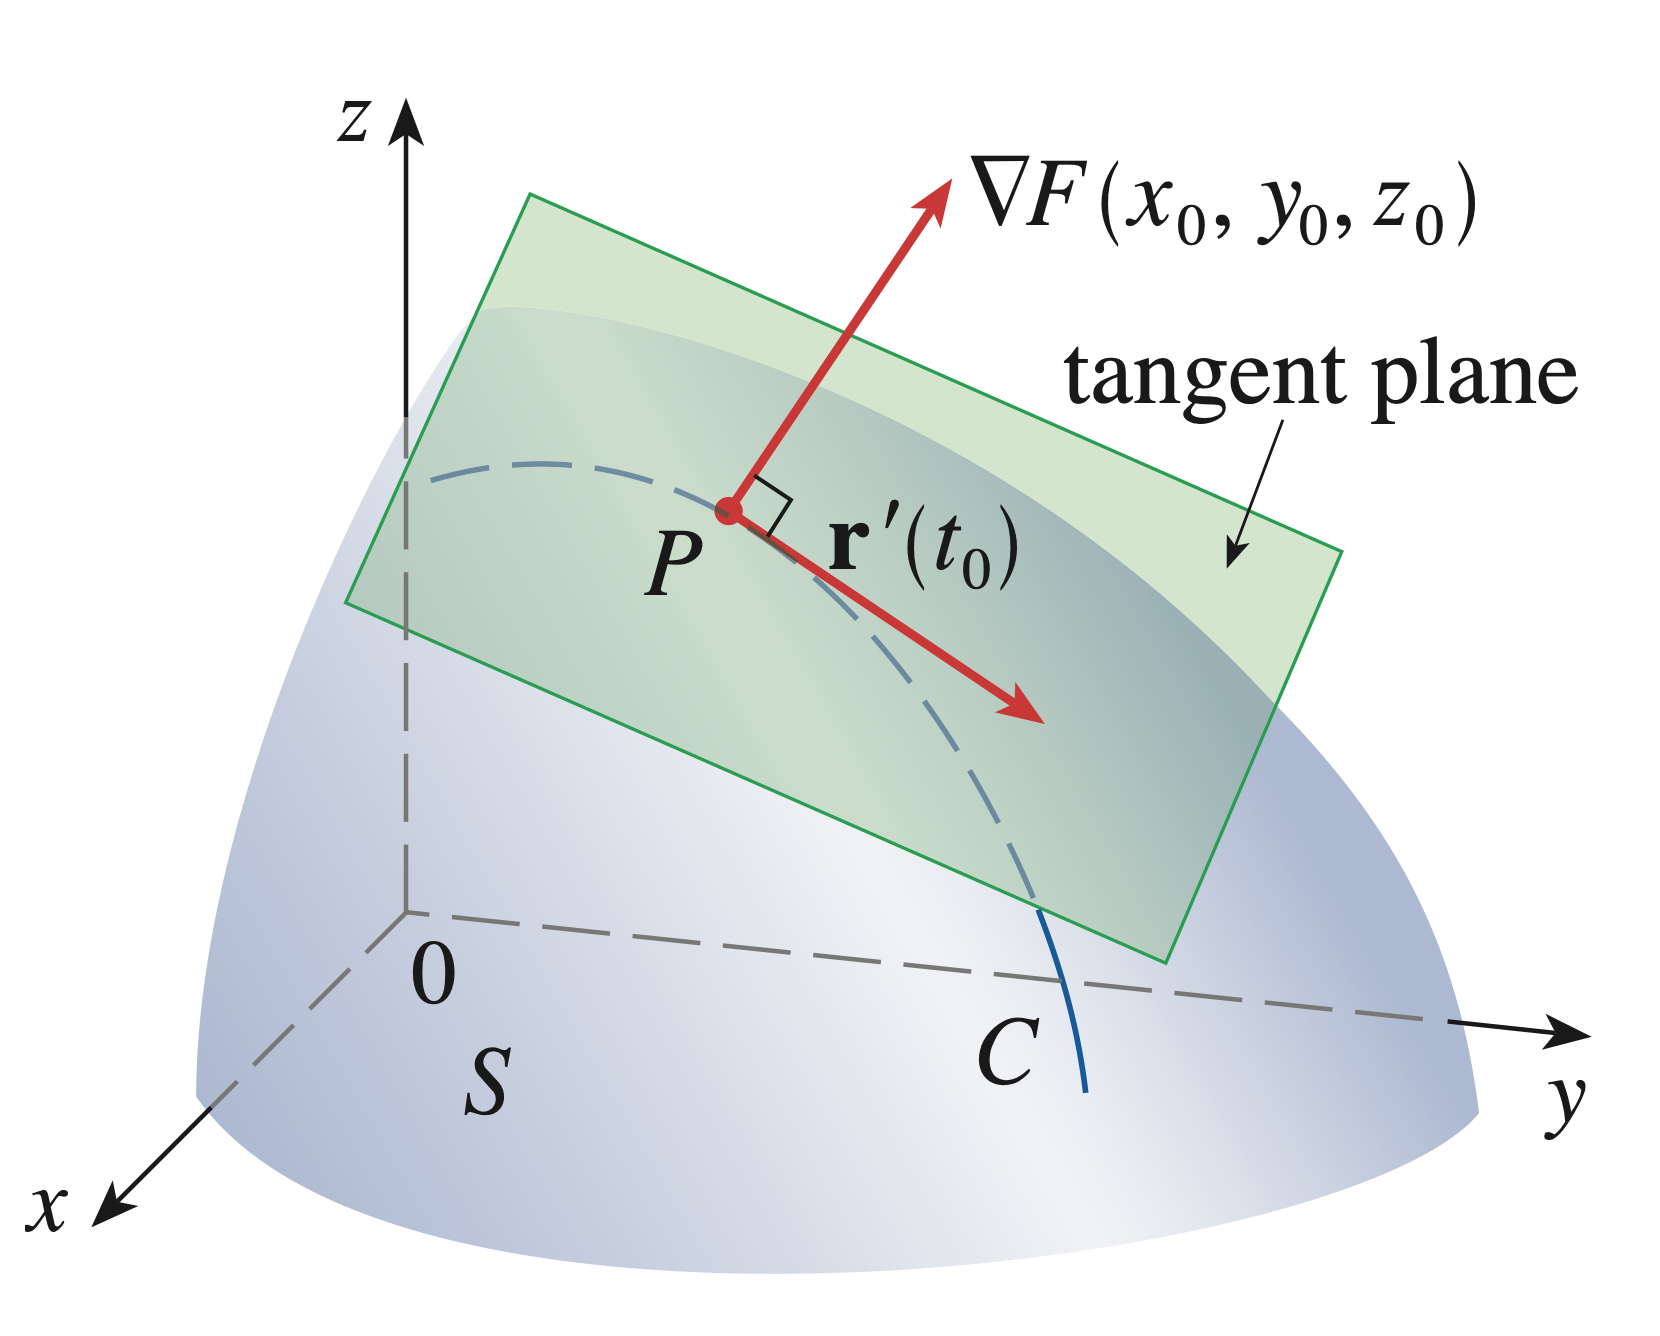
\includegraphics[scale=0.25]{TangentPlanesToLevelSurfaces}
	\]
	Because any point on the curve must satisfy the equation $F(x,y,z) = k$, we have
	$F(x(t),y(t),z(t)) = k$. Assuming that $F, f, x,y,z$ and $t$ are all
	differentiable functions we have
	\[
		\pdv{F}{x}\frac{dx}{dt}+\pdv{F}{y}\frac{dy}{dt}+ \pdv{F}{z}\frac{dz}{dt}= 0
	\]
	Notice that $\nabla F = \langle F_{x},F_{y},F_{z} \rangle$ and
	$\vec{r}\,'(t)= \langle x\,'(t),y\,'(t),z\,'(t) \rangle$ So
	\begin{align*}
		\nabla F \cdot \vv{r}'(t)                        & = 0 \\
		\nabla F(x_{0},y_{0},z_{0}) \cdot \vv{r}'(t_{0}) & = 0
	\end{align*}
	This means that the gradient vector at any point on the surface is always
	perpendicular to the direction of the tangent vector of the point on a curve
	that passes through the point.
	\begin{mybox}
		{Tangent plane to level surface} In fact, we can defined the tangent plane
		to the level surface at some point $P(x_{0},y_{0},z_{0})$ as
		\[
			F_{x}(x_{0},y_{0},z_{0})(x-x_{0}) + F_{y}(x_{0},y_{0},z_{0})(y-y_{0}) + F_{z}
			(x_{0},y_{0},z_{0})(z-z_{0}) = 0
		\]

		Astutely, we notice that this does not directly come from
		$\nabla F(x_{0},y_{0},z_{0}) \cdot \vv{r}'(t_{0}) = 0$. But the vector formed
		by some arbitrary point $P(x,y,z)$ on the tangent plane and a known point $P_{0}
		(x_{0},y_{0},z_{0})$ will always be parallel to the tangent vector of some curve
		at $(x_{0},y_{0},z_{0})$. In other words, there will always be a curve passing
		through $P_{0}$ whose tangent vector at $P_{0}$ is parallel to the vector $\overrightarrow
		{P_0P}$ If the gradient is orthogonal to the tangent vector at a known point,
		then it must also be orthogonal to the vector which is parallel to the
		tangent vector. So it is safe to say that the gradient is indeed perpendicular
		to any line on the tangent plane and thus we can define the tangent plane as
		above.
	\end{mybox}
	If we consider a function of two variables and a point $P(x_{0},y_{0})$ in the
	domain. The gradient vector at $P$, $\nabla f(x_{0},y_{0})$ is perpendicular to
	the level curve $f(x,y) = k$ that passes through $P$, in other words, its perpendicular
	to the tangent vector of the curve at $P$.
	\[
		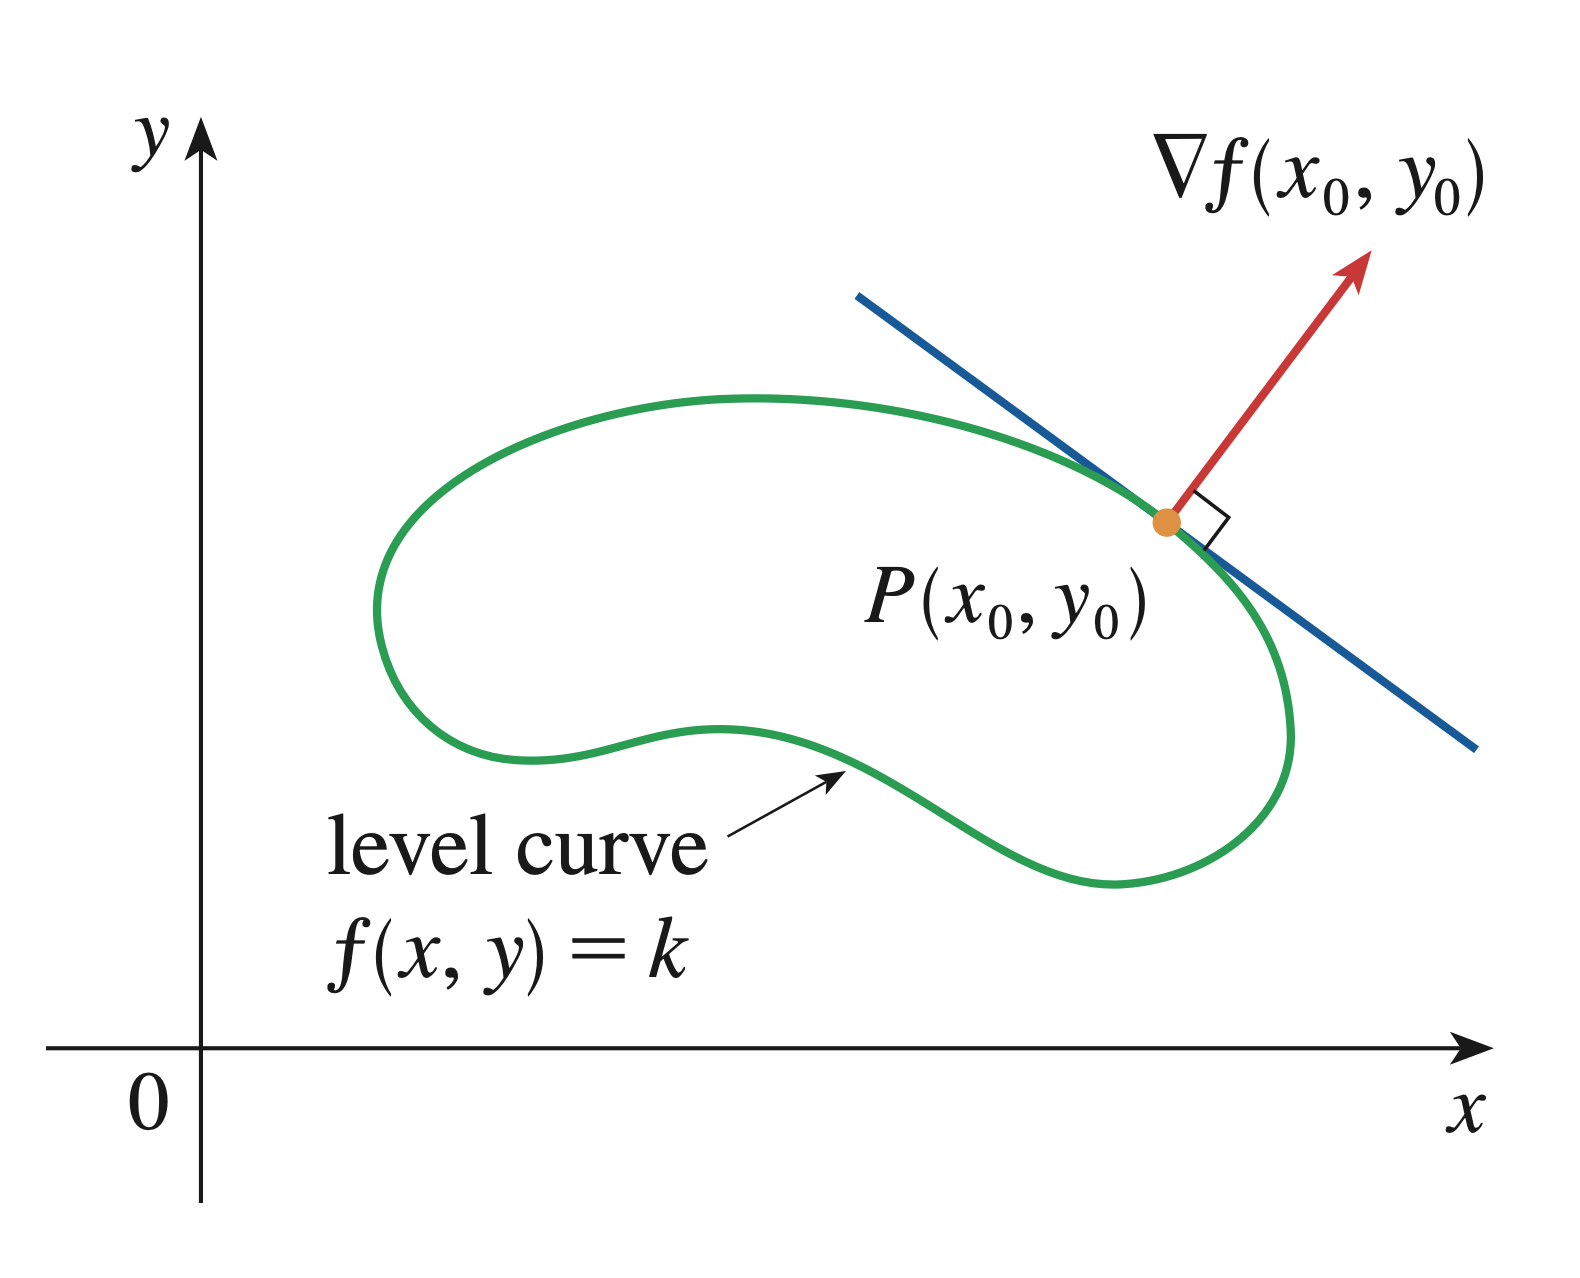
\includegraphics[scale=0.4]{OrthogonalToLevelCurve}
	\]
	\pagebreak
	\begin{mybox}
		{Properties of the Gradient Vector} Let $f$ be a differentiable function of two
		or three variables and suppose that the gradient $\nabla f(x) \not = \vec{0}$
		then we have the following three properties concerning the gradient vector at
		some point $P(x,y,z)$
		\begin{itemize}
			\item The directional derivative of $f$ at $P$ is given by $D_{u}f(x,y,z)=
				\nabla f(x,y,z) \cdot \vec{u}$

			\item $\nabla f(x,y,z)$ points in the direction of the maximum rate of increase
				of $x$ at $P$. In other words, the directional vector at $P$ is maximized
				when we it is in the direction of the gradient

			\item $\nabla f(x,y,z)$ is perpendicular to the level curve or level surface
				of $f$ through $P$
		\end{itemize}
	\end{mybox}
	\subsection{14.7 Maximum and minimum values}
	\begin{mybox}
		{Local maximums and minimums} A function of two variables has a local maximum
		at $(a,b)$ if $f(x,y) \leq f(a,b)$ when $(x,y)$ is near $(a,b)$. It has a
		local minimum at $(a,b)$ if $f(x,y) \geq f(a,b)$ when $(x,y)$ is near
		$(a,b)$.
	\end{mybox}

	For single variable function we know that if a function $f$ has a local minimum
	or maximum at $c$ and $f'(c)$ exists, then $f'(c) = 0$. Similarly, we have the
	following theorem for functions of two variables.

	\begin{mybox}
		{Critical points} If $f$ has a local maximum or minimum at $(a,b)$ and the first
		order partial derivative exists there, we have $f_{x}(a,b) = 0$ and
		$f_{y}(a,b) = 0$.
	\end{mybox}
	All local minima or maxima are critical points, but not all critical points are
	local maxima or minima. \textbf{If a critical point is neither a local maxima
	or minima, then it is a saddle point.} To determine whether a critical point is
	a local minimum or maximum or a saddle point. We have the second derivatives
	test.
	\begin{mybox}
		{Second derivatives test} Suppose the second partial derivatives of $f$ are continuous
		on a disk with center $(a,b)$ and suppose that $f_{x}(a,b)=0$ and $f_{y}(a,b)
		=0$. Let
		\[
			D=D(a,b)=f_{xx}(a,b)f_{yy}(a,b) - (f_{xy}(a,b))^{2}
		\]
	\end{mybox}
	It can also be defined as the determinant of a two by two matrix defined by the
	following
	\[
		\begin{vmatrix}
			f_{xx} & f_{xy} \\
			f_{yx} & f_{yy}
		\end{vmatrix}
	\]
	\begin{itemize}
		\item If $D>0$ and $f_{xx}(a,b) > 0$, then $f(a,b)$ is a local minimum

		\item If $D>0$ and $f_{xx}(a,b) < 0$, then $f(a,b)$ is a local maximum

		\item If $D<0$ then $(a,b)$ is a saddle point of $f$
	\end{itemize}
	\begin{mybox}
		{Absolute maximums and minimums} A function of two variables with domain $D$
		has a absolute maximum at $(a,b)$ if $f(x,y) \leq f(a,b)$ for all $(x,y) \in
		D$ It has a local minimum at $(a,b)$ if $f(x,y) \geq f(a,b)$ for all $(x,y) \in
		D$.
	\end{mybox}
	To find the absolute maximum and minimum values of a continuous function $f$ on
	a closed, bounded set $D$, we need to find the critical points of $f$ inside the
	bounded region, and then find the extreme values of $f$ at the boundary, and finally
	we compare the values that we obtained to conclude the absolute maximum and minimum
	of the function.
	\subsection{14.8 Lagrange Multipliers}
	The method of the Lagrange multipliers is a way to maximize or minimize values.
	\[
		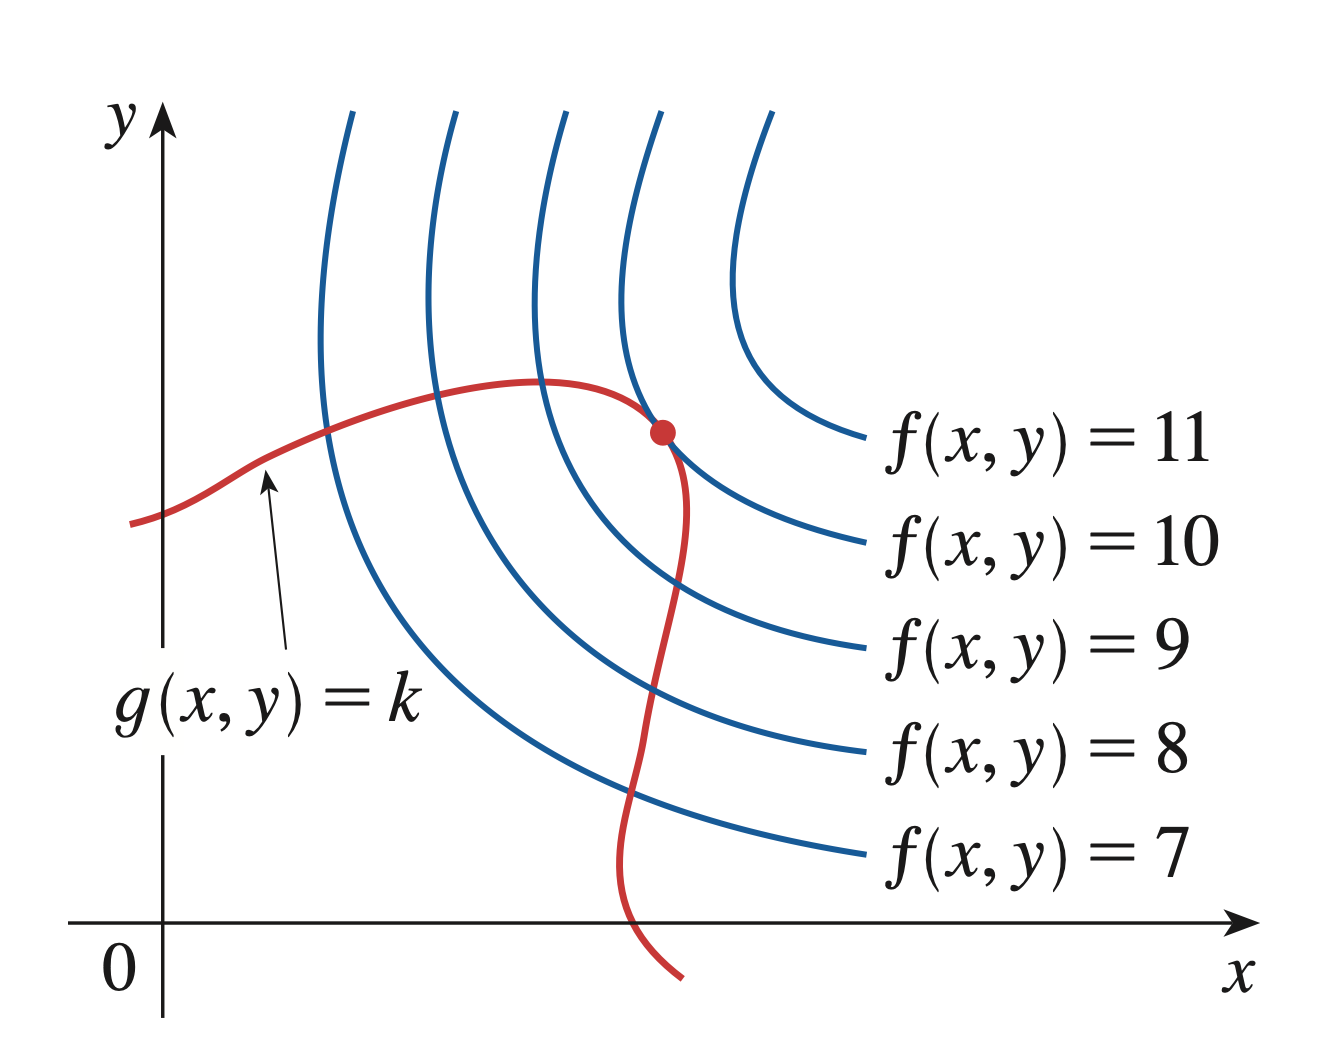
\includegraphics[scale=0.4]{Lagrange}
	\]
	Suppose we have a function $f(x,y)$ subject to a constraint of the form $g(x,y)
	= k$. If we want to seek the extreme values of $f$ we would want to seek the
	largest or smallest $f(x,y)$ while $(x,y)$ satisfies $g(x,y) = k$. Notice that
	this will always occur when the level curve $g(x,y) = k$ touches the level curves
	of $f$. Consequently, we must have $\nabla f(x,y,z) = \lambda \nabla g(x,y,z)$,
	because they would have gradient vectors that are parallel. This is extendable
	to functions of three variables which will follow a similar pattern of reasoning
	as that of functions of two variables. If the level surface of the constraint
	meet the extreme value of the function we are maximizing, it will always be such
	that their gradient vectors are parallel to each other.
	\begin{mybox}
		{Method of Lagrange Multipliers} To find the maximum and minimum values of $f
		(x,y,z)$ subject to the constraint $g(x,y,z) = k$
		\begin{itemize}
			\item We find all values of $x,y,z$ and $\lambda$ such that $\nabla f(x,y,z
				) = \lambda \nabla g(x,y,z)$ and $g(x,y,z) = k$

			\item Evaluate $f$ at all the points (x,y,z) that result from step1. The
				largest of these values is the maximum value of $f$ and the smallest is
				the minimum value of $f$.
		\end{itemize}
	\end{mybox}
	\pagebreak
	\section{15 Multiple integrals}
	\subsection{15.1 Double Integrals over Rectangles}
	Consider a function of two variables defined on a closed rectangle
	$R = \{(x,y) \in \mathbb{R}^{2} | a \leq x \leq b, c \leq y \leq d\}$
	\[
		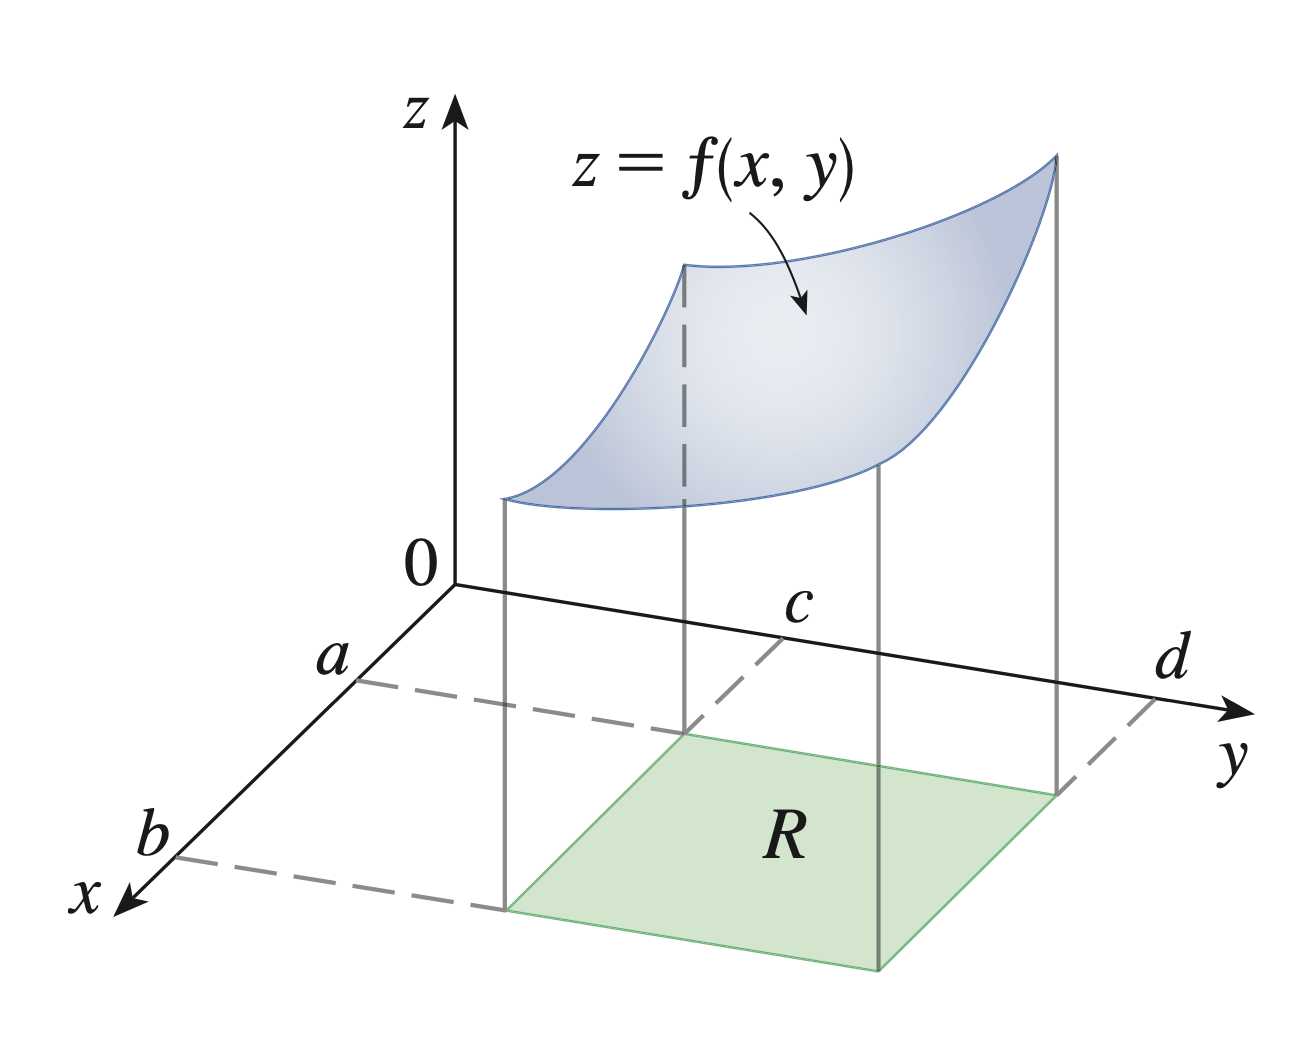
\includegraphics[scale=0.4]{VolumeUnderSurface}
	\]
	We shall follow a similar line of reasoning when finding the volume under a
	surface defined by two variables to that of finding the area under a curve. We
	shall divide the region $R$ into sub rectangles each with area $\Delta A = \Delta
	x \Delta y$. If we choose some sample point in each sub-rectangle
	$(x^{*}_{ij},y^{*}_{ij})$ then we can represent the volume under the surface
	and above each sub-rectangle as $f(x^{*}_{ij},y^{*}_{ij})\Delta A$ where
	$f(x,y)$ is the function defining the surface. The volume can thus be approximated
	by
	\[
		V \approx \sum_{i=1}^{m}\sum_{j=1}^{n}f(x^{*}_{ij},y^{*}_{ij}) \Delta A
	\]
	\[
		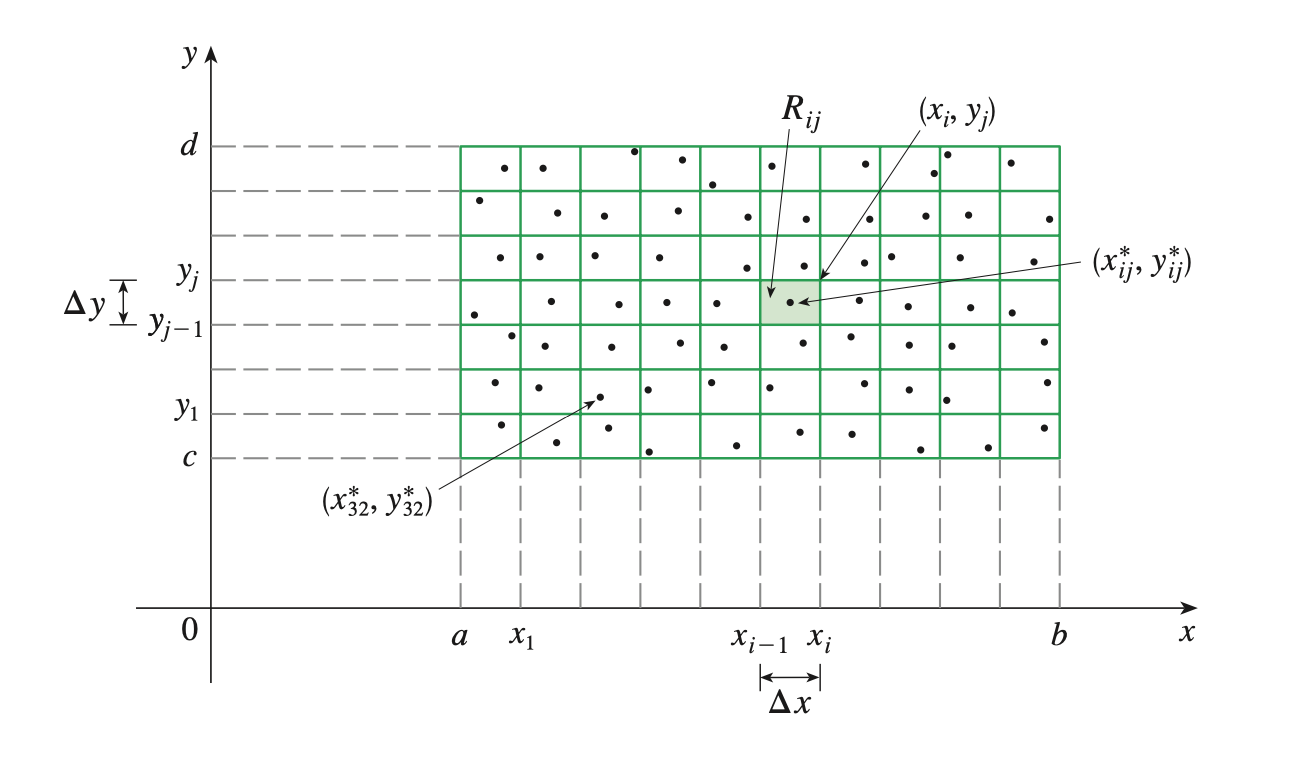
\includegraphics[scale=0.6]{DivisionInToSubRectangles}
	\]
	$m$ and $n$ would be the number of sub rectangles in the $x$ direction and the
	$y$ direction respectively. As the region is divided into $mn$ sub-rectangles,
	we would expect the sub-rectangles to get smaller as $m$ and $n$ gets larger and
	$f(x^{*}_{ij},y^{*}_{ij})$ to reflect more accurately the height of the column
	above any sub-rectangles. Finally, we have
	\[
		V = \lim_{m,n \to \infty}\sum_{i=1}^{m}\sum_{j=1}^{n}f(x^{*}_{ij},y^{*}_{ij})
		\Delta A
	\]
	\begin{mybox}
		{Double Integral Over A Region} The double integral of $f$ over the rectangle
		$R$ is
		\[
			\iint\limits_{R} f(x,y) \,dA = \lim_{m,n \to \infty}\sum_{i=1}^{m}\sum_{j=1}
			^{n}f(x_{ij},y_{ij}) \Delta A
		\]
		if the limit exists and where $(x_{ij},y_{ij})$ is any sample point inside the
		sub-squares.
	\end{mybox}
	We can evaluate these double integrals by expressing them as an iterated integral.
	\begin{mybox}
		{Double Integral As Interated Integral} The double integral of $f$ over the rectangle
		$R$ is
		\[
			\iint\limits_{R} f(x,y) \,dA = \int_{a}^{b}\int_{c}^{d}f(x,y) \, dy \, dx =
			\int_{c}^{d}\int_{a}^{b}f(x,y) \, dx \, dy
		\]
	\end{mybox}
	In the case that $f(x,y)$ can be written as the product of a function $g(x)$
	only and $h(y)$ only we have
	\[
		\iint\limits_{R} f(x,y) \,dA = \int_{a}^{b}g(x) \, dx \int_{c}^{d}h(y) \, dy
	\]
	where $R = [a,b] \times [c, d]$
	\begin{mybox}
		{Average value of a function of two variables} The average value of a function
		of two variables defined over a rectangle $R$ can be defined as
		\[
			f_{avg}= \frac{1}{A(r)}\iint\limits_{R} f(x,y) \,dA
		\]
	\end{mybox}
	\subsection{15.2 Double Integrals over General Regions}
	If we want to find the double integral of some function $f(x,y)$ over some
	general region $D$, we define a new function $F(x,y)$ which agrees with $f(x,y)$
	in the region $D$ but with domain $R$. In other words $F(x,y)= f(x,y)$ for
	$(x,y) \in D$ and $F(x,y)= 0$ for $(x,y)\not\in D$
	\[
		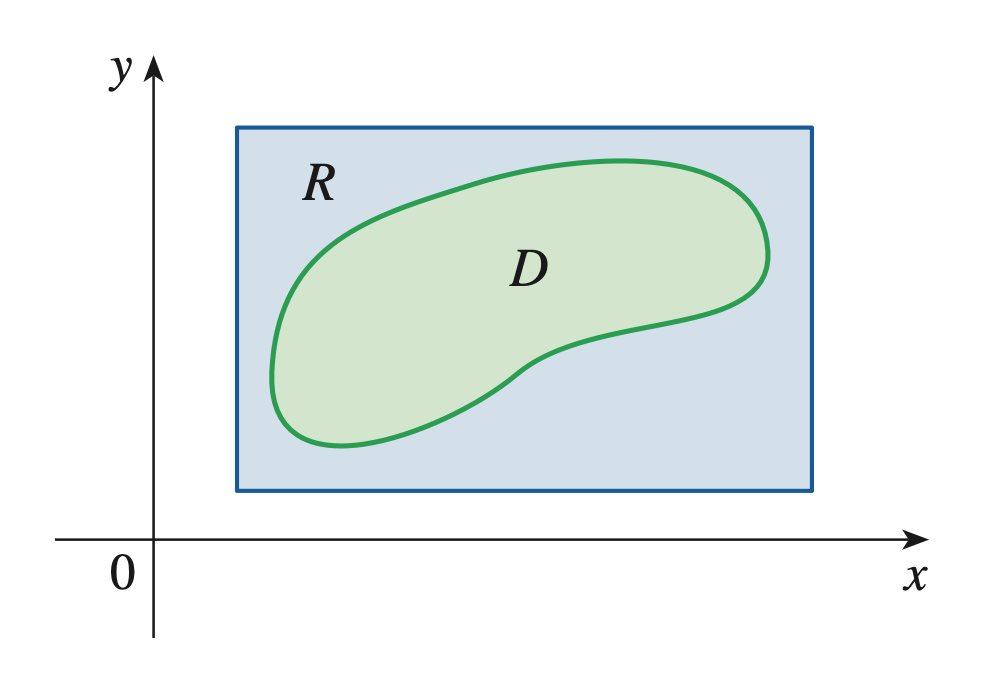
\includegraphics[scale=0.5]{F(x,y)}
	\]
	Suppose now that the region $D$ is a vertically simple region where the region
	lies between two functions of $x$. We choose a rectangle $R=[a,b] \times [c,d]$
	that contains the region $D$ and let $F(x,y)$ be defined as we defined it previously.
	By Fubini's theorem we have
	\[
		\iint\limits_{D} f(x,y) \,dA = \iint\limits_{R} F(x,y) \,dA = \int_{a}^{b}\int
		_{c}^{d}F(x,y) \, dy \, dx =\int_{a}^{b}A(x) \, dx
	\]
	\[
		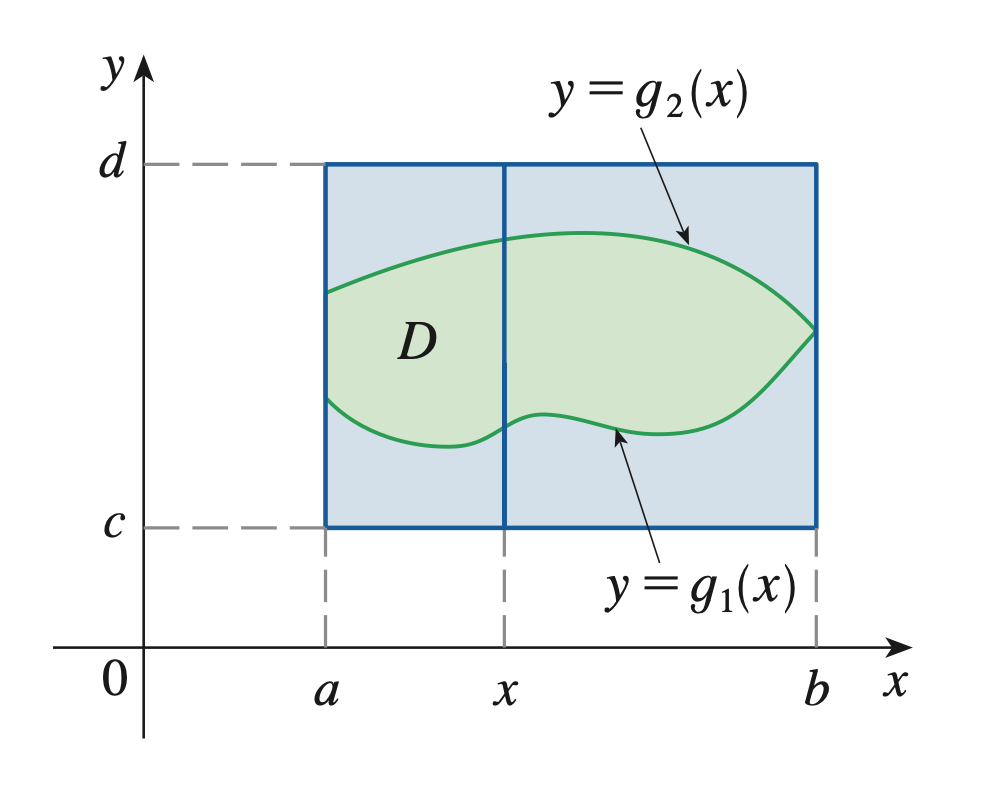
\includegraphics[scale=0.5]{VerticallySimple_1}
	\]
	Notice that beyond $g_{2}(x)$ and $g_{1}(x)$, $F(x,y) = 0$, so they contribute
	nothing to the area. So
	\[
		A(x) = \int_{c}^{d}F(x,y) \, dy = \int_{g_1(x)}^{g_2(x)}F(x,y) \, dy = \int_{g_1(x)}
		^{g_2(x)}f(x,y) \, dy
	\]
	And since the region $D$ would match the $x$ bounds of the region $R$ that contains
	it, we have
	\[
		\iint\limits_{D} f(x,y) \,dA \int_{a}^{b}\int_{g_1(x)}^{g_2(x)}f(x,y) \, dy \,
		dx
	\]
	\begin{mybox}
		{Double Integral over a vertically simple region} if $f$ is continuous on a type
		I or vertically simple region $D$ described by $D = \{(x,y)|\, a \leq x \leq
		b, \, g_{1}(x) \leq y \leq g_{2}(x) \}$
		\[
			\iint\limits_{D} f(x,y) \,dA = \int_{a}^{b}\int_{g_1(x)}^{g_2(x)}f(x,y) \,
			dy \, dx
		\]
	\end{mybox}
	By similar argument we have, for a horizontally simple, or type II region we
	have
	\begin{mybox}
		{Double Integral over a horizontally simple region} if $f$ is continuous on a
		type II or horiontally simple region $D$ described by $D = \{(x,y)|\, h_{1}(y
		) \leq x \leq h_{2}(y), \, c \leq y \leq d \}$
		\[
			\iint\limits_{D} f(x,y) \,dA = \int_{c}^{d}\int_{h_1(y)}^{h_2(y)}f(x,y) \,
			dx \, dy
		\]
	\end{mybox}
	If we integrate the function $f(x,y) = 1$ over a region $D$, we obtain the area
	$A(D)$.
	\[
		\iint\limits_{D} f(x,y) \,dA = A(D)
	\]
	\subsection{15.3 Double Integrals in Polar Coordinates}

	In order to compute the double integral $\iint_{R}f(x,y) \,dA$ where $R$ is a polar
	rectangle, we can divide the region into $m$ sub-intervals from $r=a$ to $r=b$
	with width $\Delta r$ and we divide the region further by dividing the region
	from $\theta = \alpha$ to $\theta = \beta$ with width $\delta \theta$
	\[
		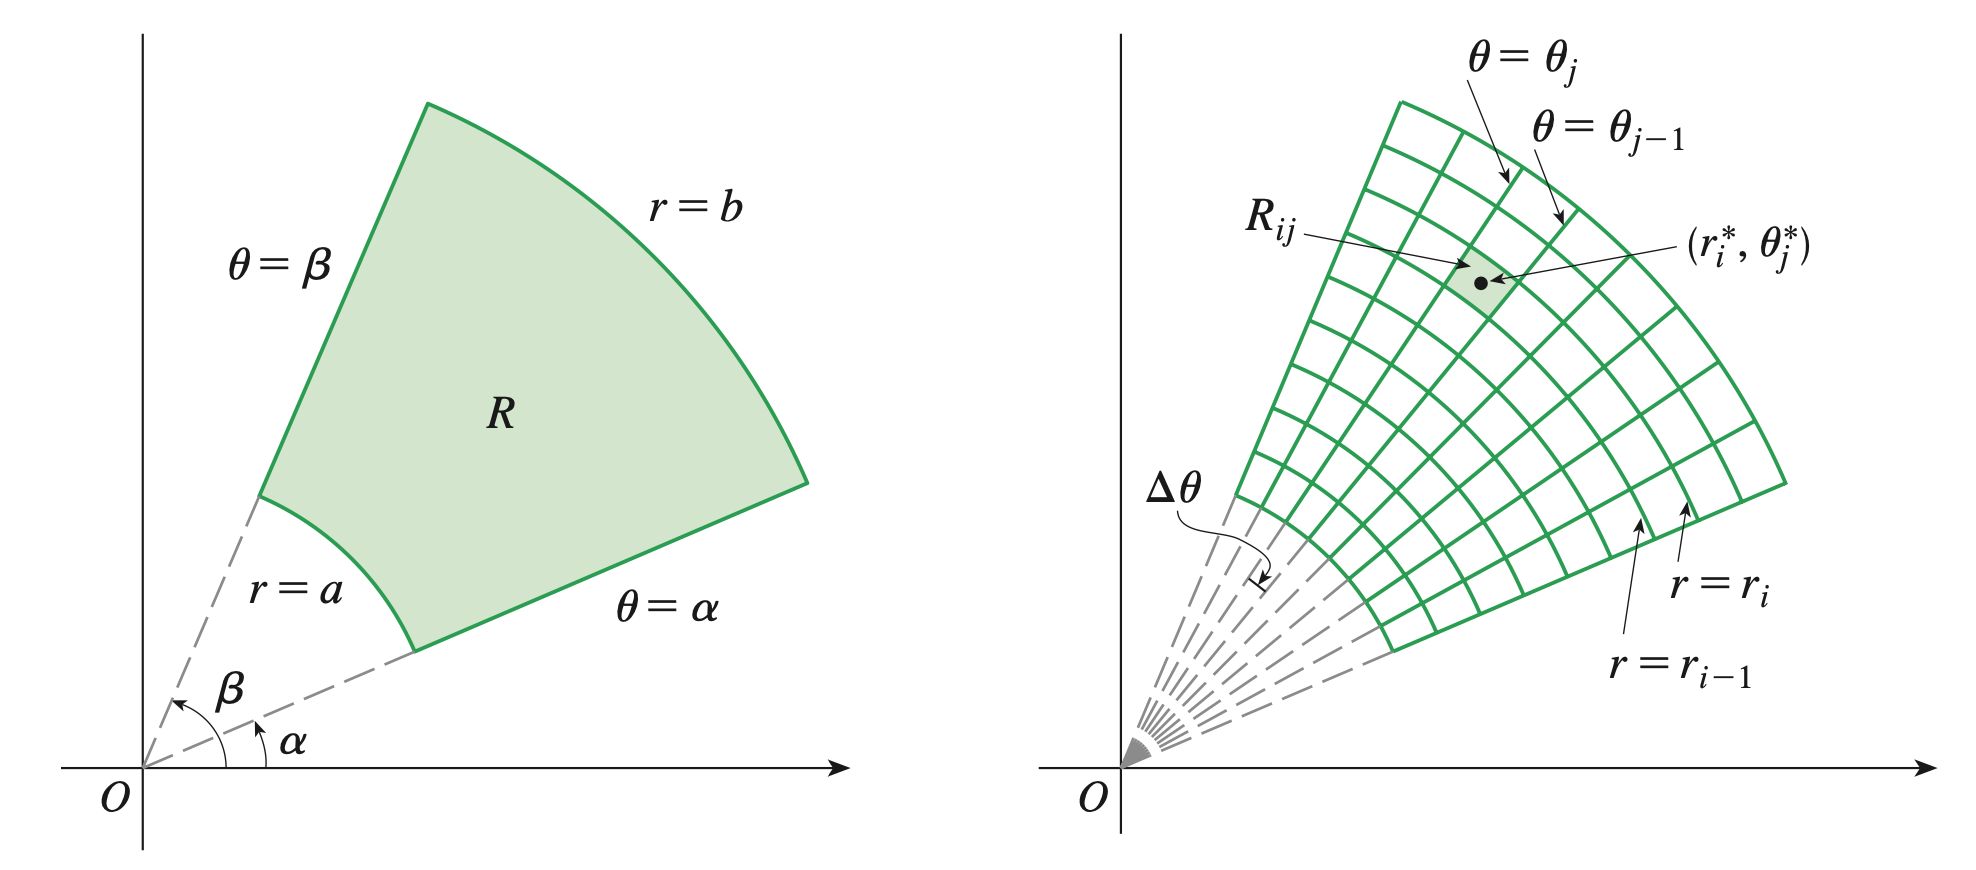
\includegraphics[scale=0.4]{PolarRectangles}
	\]
	Employing a similar approach to that of finding the double integral of a
	rectangular region, we find the area of each region and discover that it is given
	by
	\begin{align*}
		\Delta A_{i} & = \frac{1}{2}r^{2}_{i}\Delta \theta - \frac{1}{2}r^{2}_{i-1}\Delta \theta \\
		             & = r^{*}_{i} \Delta r \Delta \theta
	\end{align*}
	So we have,
	\begin{align*}
		\iint\limits_{R} f(x,y) \,dA & = \lim_{m,n \to \infty}\sum_{i=1}^{m}\sum_{j=1}^{n}f(r^{*}_{i}\text{cos}\theta^{*}_{j},r^{*}_{i}\text{sin}\theta^{*}_{j}) \Delta A \\
		                             & = \lim_{m,n \to \infty}\sum_{i=1}^{m}\sum_{j=1}^{n}g(r^{*}_{i},\theta^{*}_{j}) \Delta r \Delta \theta                              \\
		                             & = \int_{\alpha}^{\beta}\int_{a}^{b}g(r, \theta) dr d\theta                                                                         \\
		                             & = \int_{\alpha}^{\beta}\int_{a}^{b}f(r\text{cos}\theta, r\text{sin}\theta)r \, dr d\theta
	\end{align*}
	\begin{mybox}
		{Double Integral over polar region} If $f$ is continuous on a polar rectangle
		$R$ given by $0 \leq a \leq r \leq b$, $\alpha \leq \beta$ where
		$0 \leq \beta - \alpha \leq 2\pi$
		\[
			\iint\limits_{R} f(x,y) \,dA = \int_{\alpha}^{\beta}\int_{a}^{b}f(r\text{cos}
			\theta, r\text{sin}\theta)r \, dr d\theta
		\]
	\end{mybox}
	\begin{mybox}
		{Polar region where $r$ is a function of $\theta$} If $f$ is continuous on a
		polar region of the form
		\[
			D = \{(r,\theta) | \alpha \leq \theta \leq \beta, h_{1}(\theta) \leq r \leq
			h_{2}(\theta) \}
		\]
		\[
			\iint\limits_{R} f(x,y) \,dA = \int_{\alpha}^{\beta}\int_{h_1(\theta)}^{h_2(\theta)}
			f(r\text{cos}\theta, r\text{sin}\theta)r \, dr d\theta
		\]
	\end{mybox}
	In the particular case of $h_{1}(\theta) = 0$, the area of the region can be given
	by
	\begin{align*}
		\iint\limits_{D} 1 \,dA & = \int_{\alpha}^{\beta}\int_{0}^{h_2(\theta)}r \, dr d\theta                         \\
		                        & = \int_{\alpha}^{\beta}\left[ \frac{r^{2}}{2}\right]^{h_2(\theta)}_{0} \, dr d\theta \\
		                        & = \int_{\alpha}^{\beta}\frac{1}{2}\left[h(\theta)\right]^{2}\, d\theta
	\end{align*}
	\subsection{15.5 Surface Area}
	\textbf{TODO}
	\subsection{15.6 Triple Integrals}
	We can define triple integrals for functions of three variables just like we
	defined double integrals for functions of two variables. Suppose we have a function
	defined over the domain $B$, which is a rectangular box defined by
	\[
		B= \{(x,y,z)| a \leq x\leq b, c \leq y \leq d, r \leq z \leq s \}
	\]
	We then divide the box into sub boxes each of width $\Delta x$, $\Delta y$,
	and $\Delta z$. So each sub box has volume
	\[
		\Delta V = \Delta x \Delta y \Delta z
	\]While for functions of two variable, we can easily visualize that taking the
	double Riemann sum is equivalent to finding the volume of the volume under surface
	and above the region for which the function is defined, this is intuition is
	not readily available for functions of three variables. However, we can still
	think of the triple Riemann sum as analogous to that of double and single
	Riemann sums even though it is impossible for us to visualize it.
	\[
		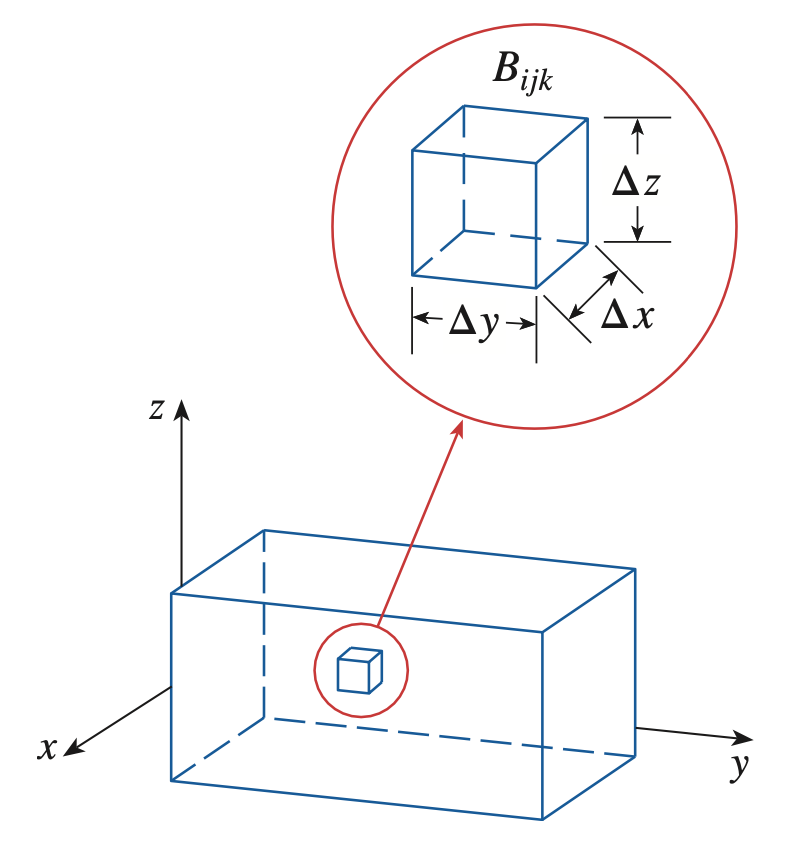
\includegraphics[scale=0.4]{Box}
	\]
	\begin{mybox}
		{Triple integral over a box} The triple integral of $f$ over the box $B$ is
		\[
			\iiint\limits_{B} f(x,y,z) dV = \lim_{l,m,n \to \infty}\sum_{i=1}^{l}\sum_{j=1}
			^{m}\sum_{k=1}^{n}f(x_{ijk},y_{ijk},z_{ijk}) \Delta V
		\]
		if the limit exists and and where $(x_{ijk},y_{ijk},z_{ijk})$ is any sample point
		inside the sub-boxes.
	\end{mybox}

	\begin{mybox}
		{Fubini's Theorem for triple integrals} If $f$ is continuous on the rectangular
		box $B = [a,b] \times [c,d] \times [r,s]$ then
		\[
			\iiint\limits_{B} f(x,y,z) dV = \int_{r}^{s}\int_{c}^{d}\int_{a}^{b}f(x,y)
			\, dx \, dy \,dz
		\]
	\end{mybox}
	For a vertically simple solid region $E$ where
	$u_{1}(x,y) \leq z \leq u_{2}(x,y)$ and $(x,y) \in D$ we have
	\[
		\iiint\limits_{E} f(x,y,z) dV = \iint\limits_{D} \left[ \int_{u_1(x,y)}^{u_2(x,y)}
		f(x,y,z) \,dz \right] \, dA
	\]
	\[
		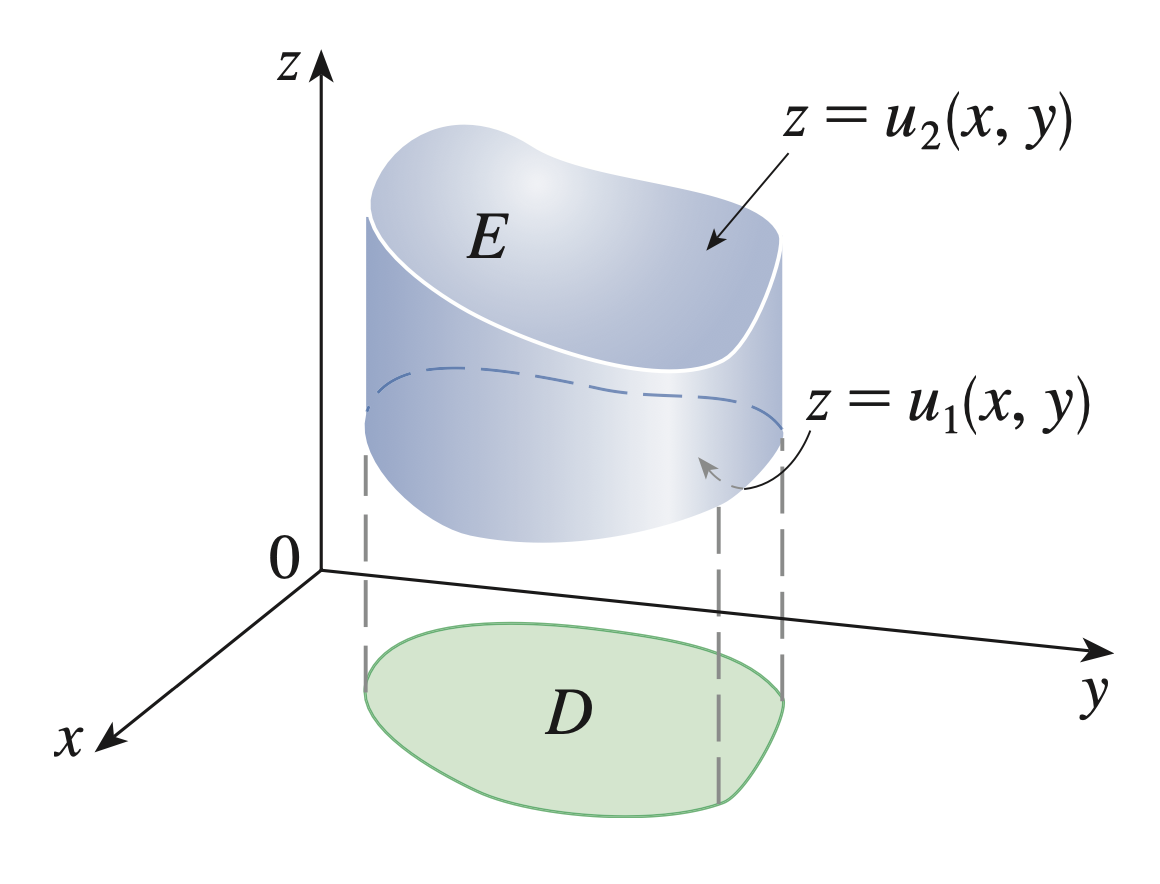
\includegraphics[scale=0.5]{Type1Solid}
	\]
	If the projection $D$ of $E$ onto the $xy$ plane has
	$g_{1}(x) \leq y \leq g_{2}(x)$ then
	\[
		\iiint\limits_{E} f(x,y,z) dV = \int_{r}^{s}\int_{g_1(x)}^{g_2(x)}\int_{u_1(x,y)}
		^{u_2(x,y)}f(x,y,z) \,dz \, dy \, dx
	\]
	\[
		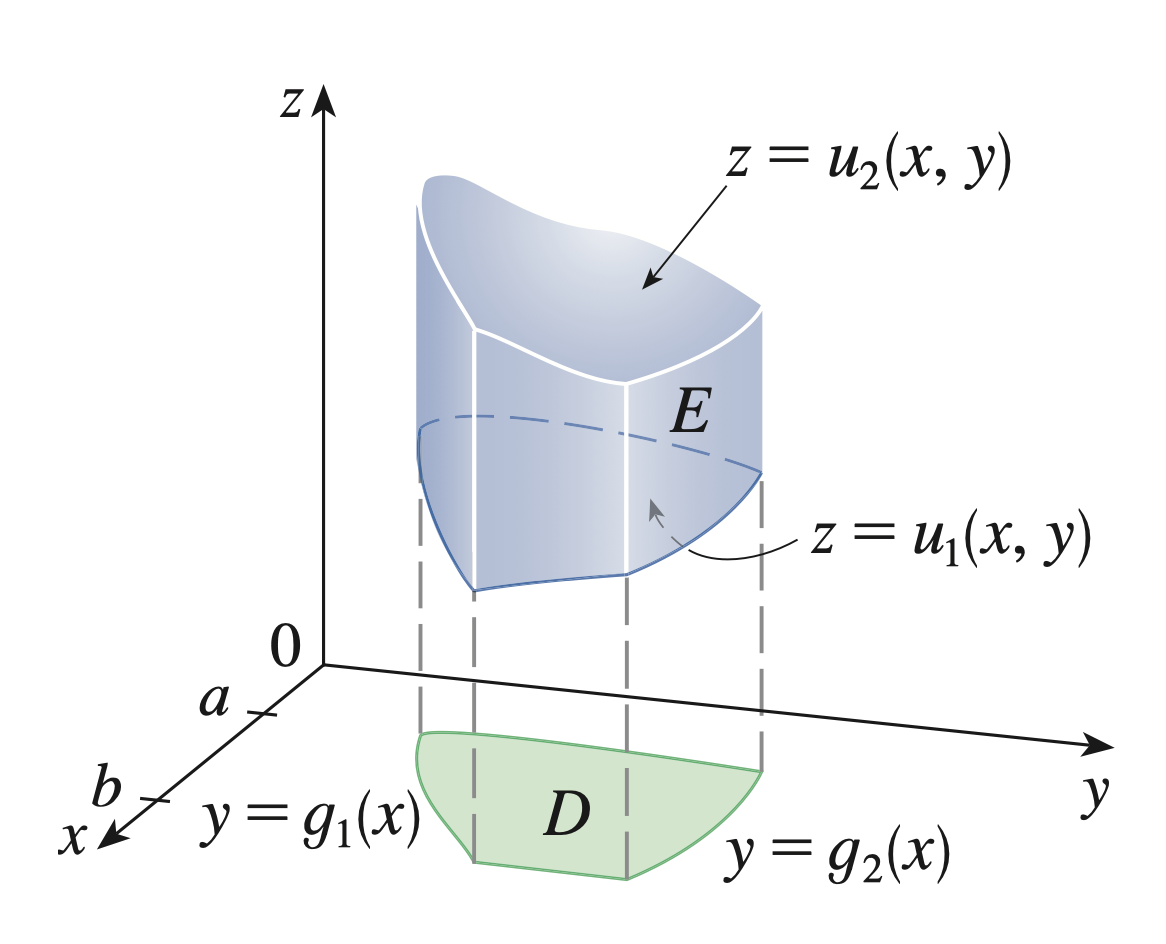
\includegraphics[scale=0.5]{Type1_1Solid}
	\]
	Naturally then, if the projection of $E$ onto the $xy$ plane has $h_{1}(x) \leq
	x \leq h_{2}(x)$ then
	\[
		\iiint\limits_{E} f(x,y,z) dV = \int_{c}^{d}\int_{h_1(x)}^{h_2(x)}\int_{u_1(x,y)}
		^{u_2(x,y)}f(x,y,z) \,dz \, dx \, dy
	\]
	\[
		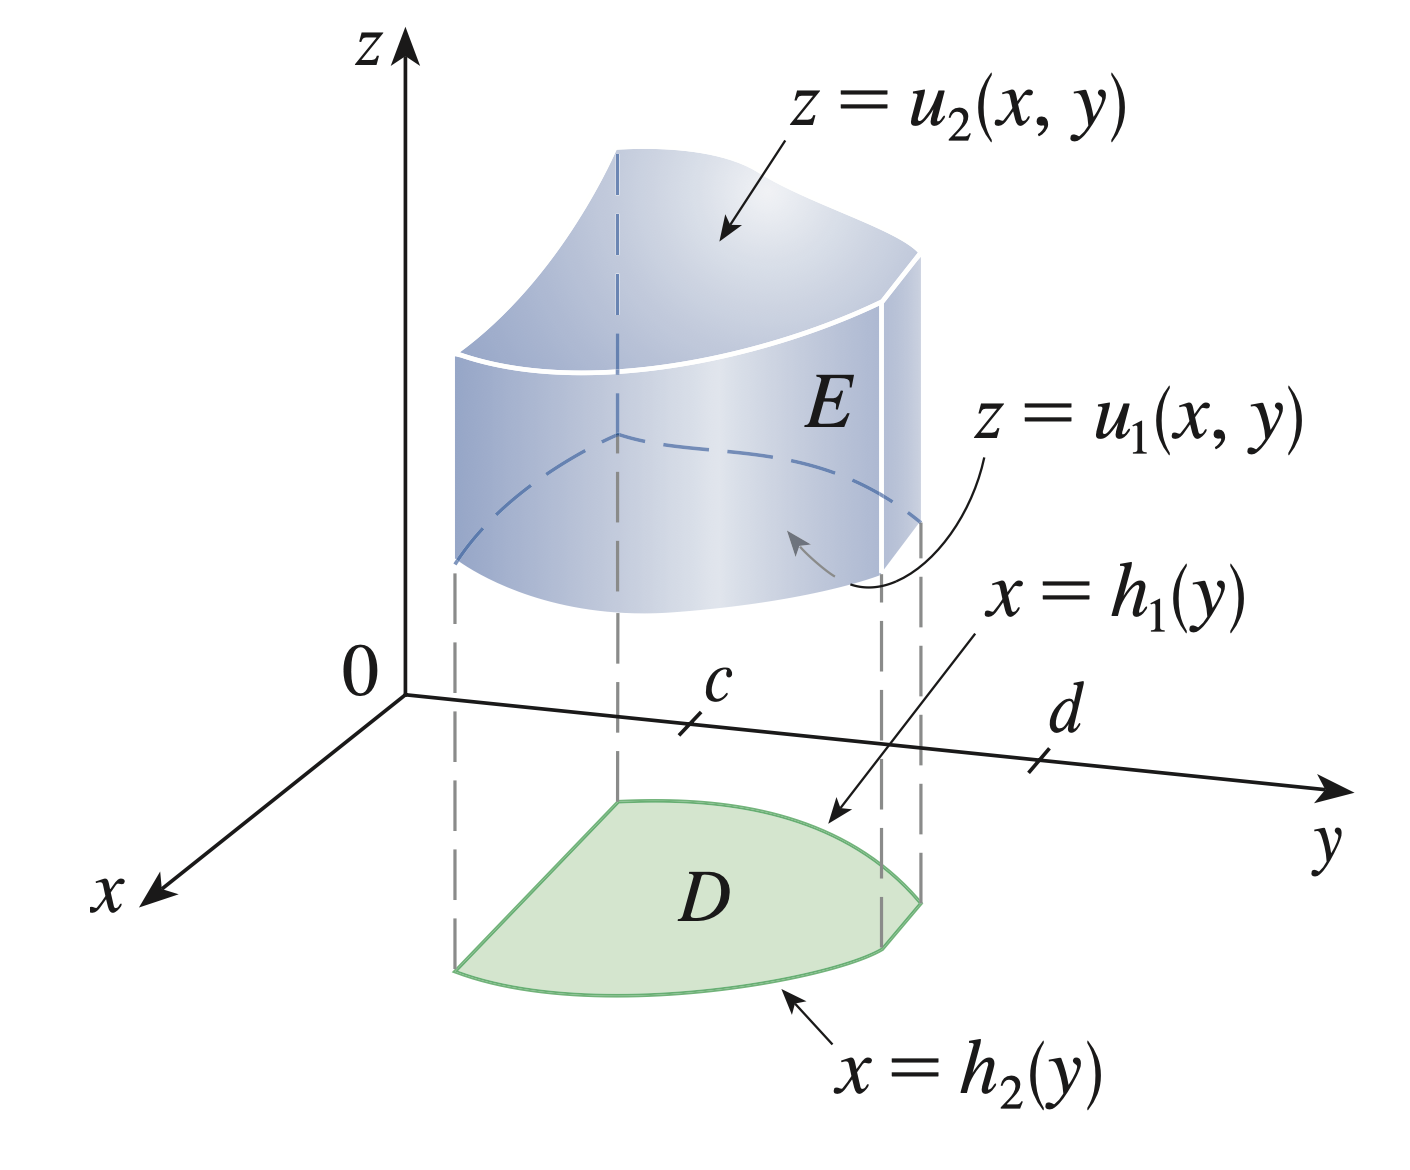
\includegraphics[scale=0.5]{Type1_2Solid}
	\]
	A type 2 region and a type 3 region are defined similarly as that of a type 3 region.
	A type 2 region is a region where the $x$ values of the solid region is
	bounded by two functions which can be expressed as function of $y$ and $z$, that
	is to say $u_{1}(y,z) \leq x \leq u_{2}(y,z)$. Similarly, for a type 3 region we
	have $u_{1}(y,z) \leq y \leq u_{2}(y,z)$. For each type of solid region, its projection
	onto the $xy$ plane can either be vertically simple or horizontally simple. If
	$f(x,y,z) = 1$, then the volume of a solid region $E$ can be given by the triple
	integral over the region $E$ with respect to the volume of the region.
	\[
		V(E) =\iiint\limits_{E} dV
	\]
	\newpage
	\subsection{15.9 Change of variables in multiple integrals}
	In section 5, we considered $u$ substitutions. By expressing a variable $x$ in
	terms of some variable $u$, we were able to simplify integrands that were a function
	of $x$. More generally, we can consider a change of variables as a transformation
	from the $uv$ plane to the $xy$ plane:
	\[
		T(u,v) = (x,y)
	\]
	where $x=x(u,v)$ and $y=y(u,v)$. If the transformation is one-to-one, there
	will be an inverse transformation. \\ Consider a transformation $T$ under which
	$S$ is transformed into $R$. The vector
	\[
		\boldsymbol{r}(u,v) = g(u,v)\boldsymbol{i}+ h(u,v)\boldsymbol{j}
	\]
	\[
		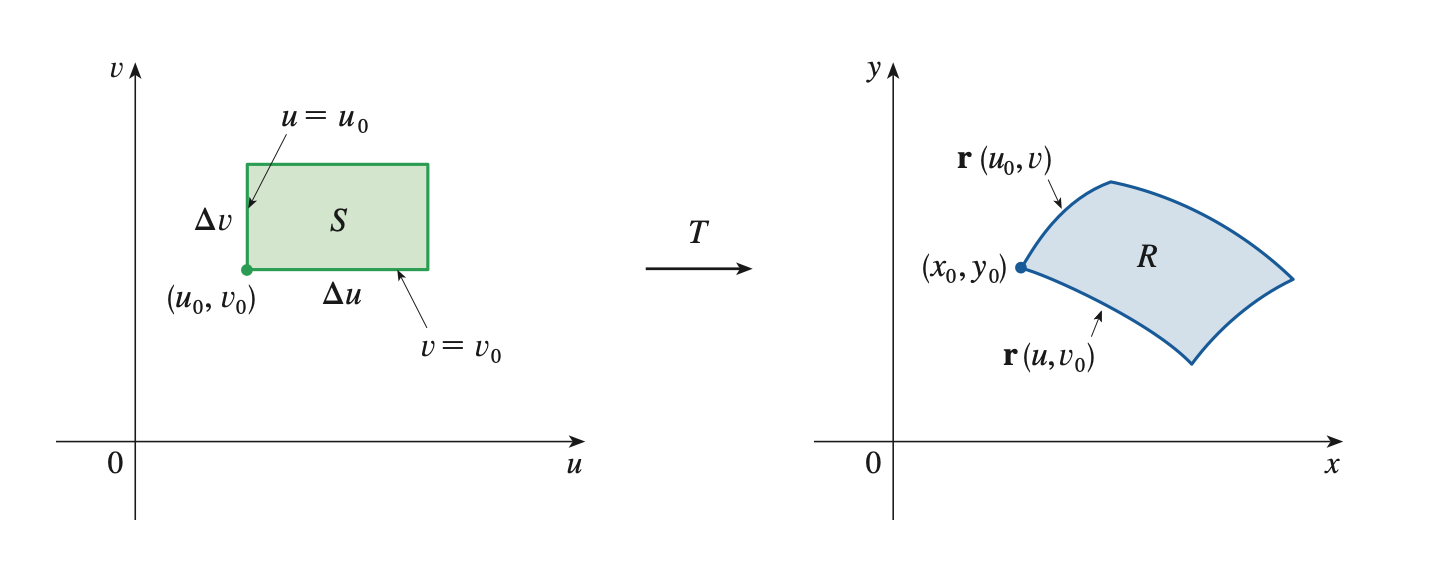
\includegraphics[scale=0.8]{Transformation}
	\]
	We can evaluate the area of a plane after transformation by a parallelogram
	\[
		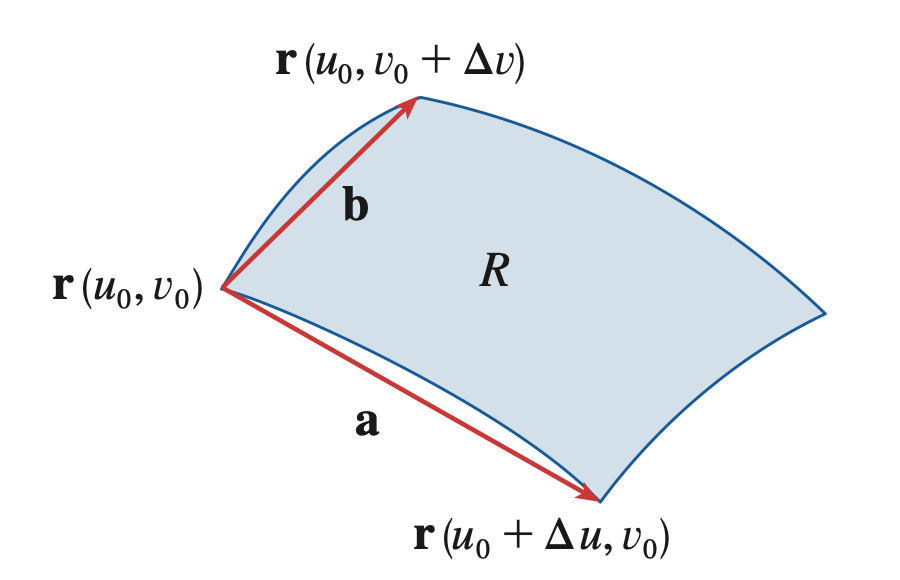
\includegraphics[scale=0.6]{Jacobian}
	\]
	Notice that, however, that
	\[
		\boldsymbol{r}_{u} = \lim_{\Delta u \to 0}\frac{\boldsymbol{r}(u_{0}+\Delta
		u, v_{0})- \boldsymbol{r}(u_{0},v_{0})}{\Delta u}
	\]
	where $\boldsymbol{r}_{u}$ is the partial derivative of $r$ with respect to
	$u$, hence we have
	\[
		\boldsymbol{r}(u_{0}+\Delta u, v_{0})- \boldsymbol{r}(u_{0},v_{0}) \approx \Delta
		u \,\boldsymbol{r}_{u}
	\]
	By similar reasoning we have
	\[
		\boldsymbol{r}(u_{0}, v_{0}+\Delta v)- \boldsymbol{r}(u_{0},v_{0}) \approx \Delta
		v\,\boldsymbol{r}_{v}
	\]
	We know that the area of a parallelogram can be approximated by the cross product
	of two vectors that form adjacent sides of the parallelogram, so we have
	\[
		\left | \Delta v \,\bm{r}_{v} \times \Delta u \,\boldsymbol{r}_{u} \right | =
		\left | \bm{r}_{v} \times \boldsymbol{r}_{u} \right | \Delta u \, \Delta v
	\]. The cross product gives us,

	\begingroup
	\renewcommand*{\arraystretch}{1.55}
	\[
		\bm{r}_{u} \times \bm{r}_{v} =
		\begin{vmatrix}
			\bm{i}     & \bm{j}     & \bm{k} \\
			\pdv{x}{u} & \pdv{y}{u} & 0      \\
			\pdv{x}{v} & \pdv{y}{v} & 0      \\
		\end{vmatrix}
		=
		\begin{vmatrix}
			\pdv{x}{u} & \pdv{y}{u} \\
			\pdv{x}{v} & \pdv{y}{v} \\
		\end{vmatrix}\bm{k}=
		\begin{vmatrix}
			\pdv{x}{u} & \pdv{x}{v} \\
			\pdv{y}{u} & \pdv{y}{v} \\
		\end{vmatrix}\bm{k}
	\]
	\endgroup

	\begin{mybox}
		{Jacobian of a transformation $T$} The \textbf{Jacobian} of a transformation
		$T$ given by $x=g(u,v)$ and $y=h(u,v)$ is \begingroup
		\renewcommand*{\arraystretch}{1.55}
		\[
			\frac{\partial (x,y)}{\partial (u,v)}=
			\begin{vmatrix}
				\pdv{x}{u} & \pdv{x}{v} \\
				\pdv{y}{u} & \pdv{y}{v} \\
			\end{vmatrix}
		\]
		\endgroup
	\end{mybox}
	\newpage
	\section{16 Vector Calculus}
	\subsection{16.1 Vector Fields}
	\begin{mybox}
		{Vector field in space}Let $E$ be a subset of $\mathbb{R}^{3}$. A vector field
		on $\mathbb{R}^{3}$ is a function $\vec{F}$ that assigns to each point $(x,y,
		z)$ in $E$ a three-dimensional vector $\vec{F}(x,y,z)$ where
		\[
			\vec{F}(x,y,z) = P(x,y,z)\vec{i}+ Q(x,y,z)\vec{j}+ R(x,y,z)\vec{k}
		\]
	\end{mybox}
	The gradient $\nabla f$ of some function $f$ is also, in fact, a vector field
	since it assigns to every point on the domain of $f$ a vector. \\\\A vector field
	$\vec{F}$ is called a conservative vector field if it is the gradient of some scalar
	function. In other words, if there exists a function $f$ such that $\vec{F}= \nabla
	f$. $f$ can be called the potential function of $f$.
	\subsection{16.2 Line Integrals}
	The line integral of some function $f$ along some curve $C$ can be defined along
	he similar line of thought of ordinary integrals. We can divide the curve into
	small sub arcs and by making the width of these sub arcs infinitely small we
	can find the value of a function summed over that region. Divide the parameter
	interval into $n$ sub intervals $[t_{i-1},t_{i}]$, the corresponding $x$ and
	$y$ values for all parameters $t$ will divide the curve into $n$ sub arcs or
	intervals. Taking the mid point of each interval and multiplying them by the length
	of the sub arc we obtain an approximate value for the function integrated over
	the region. The larger $n$ gets the shorter the sub-arc gets and consequently,
	the more accurate our approximation of the actual value of the integral is.

	\[
		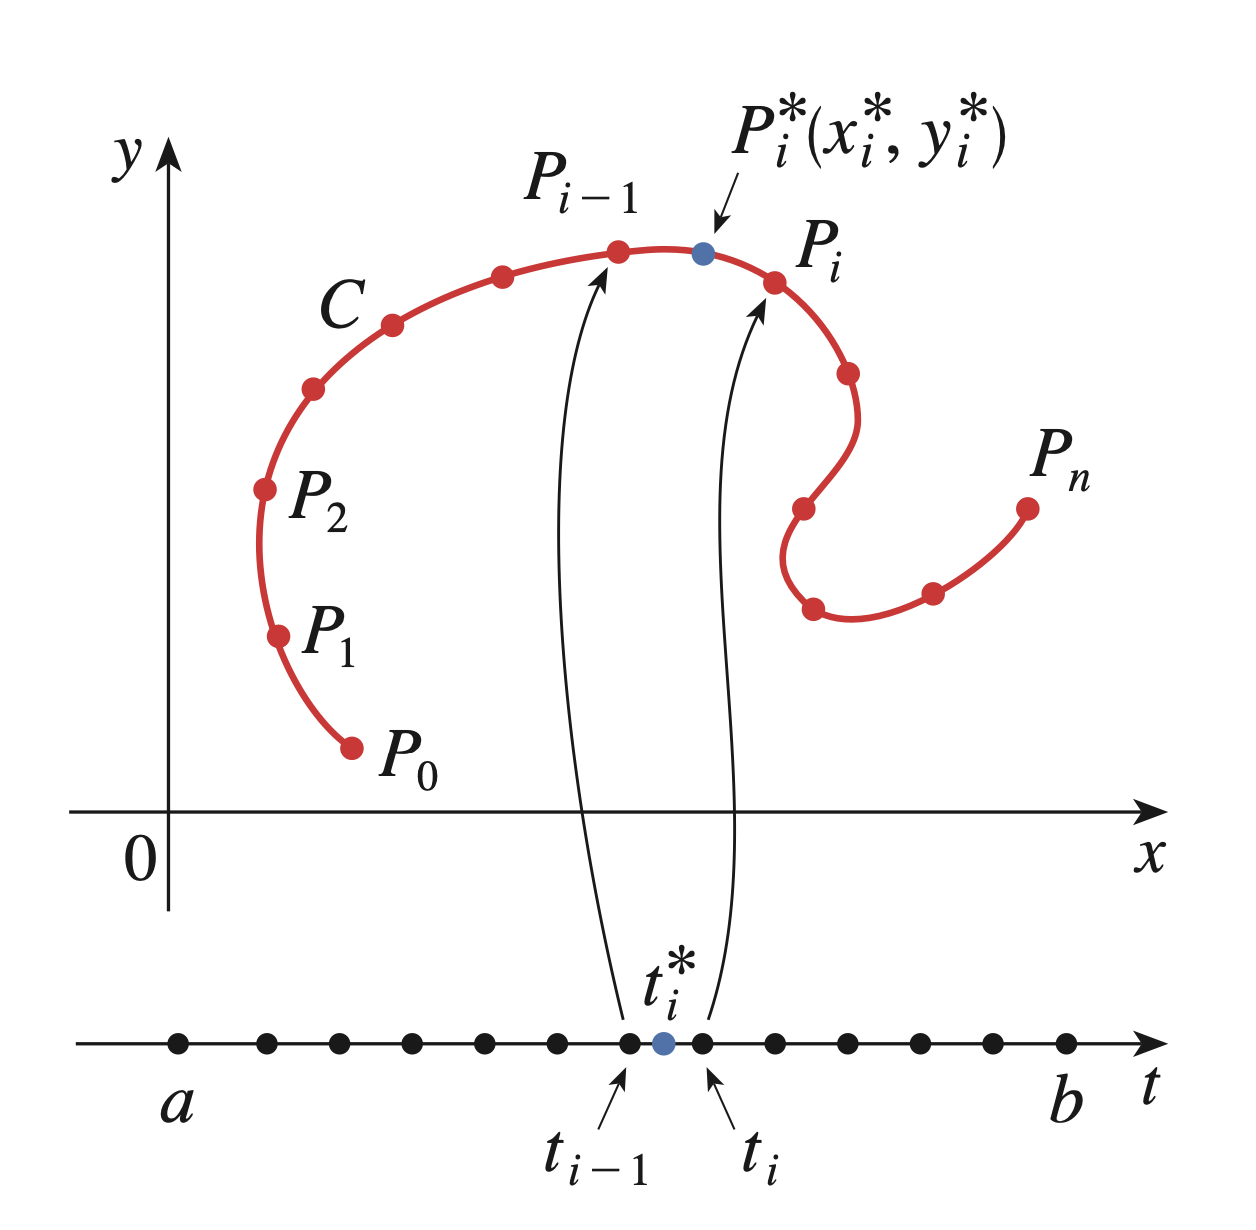
\includegraphics[scale=0.4]{LineIntegrals}
	\]
	\begin{mybox}
		{Line integrals along $C$} If $f$ is defined on a smooth curve $C$ where $x=x
		(t)$, $y=y(t)$ and $a\leq t \leq b$, then the line integral of $f$ along $C$
		is
		\[
			\int_{C} f(x,y)ds = \lim_{n \to \infty}\sum_{i=1}^{n}f(x_{i}^{*}, y_{i}^{*}
			) \Delta s_{i}
		\]
		and it can be shown that
		\[
			\int_{C} f(x,y)ds = \int_{a}^{b} f(x(t),y(t))\sqrt{(\frac{dx}{dt})^{2} + (\frac{dy}{dt})^{2}
			}dt
		\]
	\end{mybox}

	If $C$ is a piece-smooth curve, where $C$ can be segmented into $n$ smooth curves,
	then we have
	\[
		\int_{C} f(x,y)ds = \int_{C_1}f(x,y)ds + \int_{C_2}f(x,y)ds + ...+ \int_{C_n}
		f(x,y)ds
	\]

	We can also have line integrals with respect to $x$ or with respect to $y$ by replacinhg
	$\Delta s_{i}$ with either $\Delta x_{i} = x_{i} - x_{i-1}$ or with $\Delta y_{i}
	= y_{i} - y_{i-1}$

	\begin{mybox}
		{Line integral with respect to $x$ and $y$} The line integral with respect to
		$x$ and $y$ are given by
		\[
			\int_{C} f(x,y)dx = \int_{a}^{b} f(x(t),y(t))x\,'(t)dt
		\]
		\[
			\int_{C} f(x,y)dy = \int_{a}^{b} f(x(t),y(t))y\,'(t)dt
		\]
	\end{mybox}

	We can find parametrization of a line segment easily by the equation
	\[
		\vec{r}(t) = (1-t)\vec{r_0}+t\vec{r_1}
	\]
	where $\vec{r}(t)$ is the vector equation of the line and $\vec{r_0}$,
	$\vec{r_1}$ are the starting point and end point of the line segment
	respecitively. \\\\ In general, if $-C$ denotes the curve consisting of the same
	points as a curve $C$ but with initial point $B$ and end points $A$ we have

	\[
		\int_{-C}f(x,y)dx = - \int_{C}f(x,y)dx
	\]

	This is also true for line integrals with respect to $y$. However, if we integrate
	with respect to the arc length we do not change the value of the integral.
	\[
		\int_{-C}f(x,y)ds = \int_{C}f(x,y)ds
	\]
	Similarly, we have if a smooth space curve is defined by some vector function $\vec
	{r}(t)$ we have
	\[
		\int_{C} f(x,y,z) = \int_{a}^{b} f(x(t),y(t),z(t))ds = \int_{a}^{b} f(\vec{r}
		(t))|\vec{r}\,'(t)|dt
	\]

	We defined the work done $\bm{W}$ by the force field $\bm{F}$ as the limit of
	the Reimann sums
	\[
		W = \int_{C} \bm{F}\cdot \bm{T}ds = \lim_{n \to \infty}\sum_{i=1}^{n}\bm{F}(x
		_{i}^{*}, y_{i}^{*}, z_{i}^{*}) \cdot \bm{T}(x_{i}^{*}, y_{i}^{*}, z_{i}^{*})
		\Delta s_{i}
	\]
	but
	\[
		\bm{T}= \frac{\bm{r}\,'(t)}{|\bm{r}\,'(t)|}
	\]
	so
	\[
		W = \int_{C} \bm{F}\cdot \bm{T}ds = \int_{a}^{b} \left[ \bm{F}(\bm{r}(t)) \cdot
		\frac{\bm{r}\,'(t)}{|\bm{r}\,'(t)|}\right] |\bm{r}\,'(t)| dt = \int_{a}^{b} \bm
		{F}(\bm{r}(t)) \cdot \bm{r}\,'(t) dt
	\]

	This is often abbreviated As W =
	\[
		\int_{a}^{b} \bm{F}(\bm{r}(t)) \cdot \bm{r}\,'(t) dt = \int_{C} \bm{F}\cdot d
		\bm{r}
	\]

	We also have
	\[
		\int_{C} \bm{F}\cdot d\bm{r}= \int_{C} Pdx + Qdy + Rdz \text{ where }\bm{F}=
		P\bm{i}+ Q\bm{j}+ R\bm{k}
	\]

	\subsection{16.3 The Fundamental Theorem for Line Integrals}

	\begin{mybox}
		{The Fundamental Tehorem for Line Integrals} Let $C$ be a smooth curve given
		by the vector function $\vec{r}(t)$ for $a \leq t \leq b$. Let $f$ be
		differentiable and a function of two or three variables whose gradient
		vector $\nabla f$ is continous on $C$. Then

		\[
			\int_{C} \nabla f \cdot d\bm{r}= f(\bm{r}(b))- f(\bm{r}(a))
		\]
	\end{mybox}

	This theorem tells us that if a vector field is a conservative vector field(it
	is the gradient vector field of some scalar function). Then its line integral is
	the net change of its potential function at the end points of the space curve.
	It also tells us that the line integral of a conservative function is
	independent of path. That is if $C_{1}$ and $C_{2}$ are two curves with the same
	end point then
	\[
		\int_{C_1}\nabla f \cdot d\bm{r}= \int_{C_2}\nabla f \cdot d\bm{r}= f(x_{2},y
		_{2},z_{2}) - f(x_{1},y_{1},z_{1})
	\]

	\begin{mybox}
		{Independence of path and closed paths} $\int_{C}\nabla f \cdot d\bm{r}$ is independent
		of path in $D$ if and only if $\int_{C}\nabla f \cdot d\bm{r}= 0$ for every closed
		path $C$ in $D$, where a closed path refers to a path that has the same end
		point as the start point.
	\end{mybox}

	\begin{mybox}
		{Independence of path and conservative vector fields} It can be demonstrated
		that if $\int_{C}\bm{F}\cdot d\bm{r}$ is independent of path in $D$ then $\bm
		{F}$ is a conservative vector field on $D$ for a open connected region.
	\end{mybox}

	Let $F$ be some vector field defined by $\bm{F}= P\bm{i}+ Q\bm{j}$ on an open
	connected region. If $\pdv{P}{y}= \pdv{Q}{x}$ then $\bm{F}$ is a conservative vector
	field. This is usually only the case for open connected regions. Generally, if
	a field is conservative then $\pdv{P}{y}= \pdv{Q}{x}$ will hold by Clairaut's
	theorem.
	\subsection{16.4 Green's theorem}
	\begin{mybox}
		{Green's theorem} Let $C$ be a positively oriented, piecewise-smooth, simple
		closed curve in the plane and let $D$ be the region bounded by $C$. If $P$
		and $Q$ have continuous partial derivatives on an open region that contains
		$D$, then
		\[
			\int_{C} \bm{F}\cdot d\bm{r}= \int_{C} Pdx+ Qdy = \iint\limits_{D} (\pdv{Q}
			{x}-\pdv{P}{y}) dA
		\]
		for some vector field $\bm{F}= \langle P, Q \rangle$
	\end{mybox}
	It's possible to employ Green's theorem in the calculation of areas, if we
	make the integrand $\pdv{Q}{x}-\pdv{P}{y}= 1$. There are many selection of $P$
	and $Q$ such that $\pdv{Q}{x}-\pdv{P}{y}= 1$, here we shall use $P(x,y)=0$ and
	$Q(x,y)= x$, so we have
	\[
		A = \oint_{C} x dy = \iint\limits_{C} \pdv{Q}{x}-\pdv{P}{y}dA = \iint\limits_{C}
		1 dA
	\]
	\[
		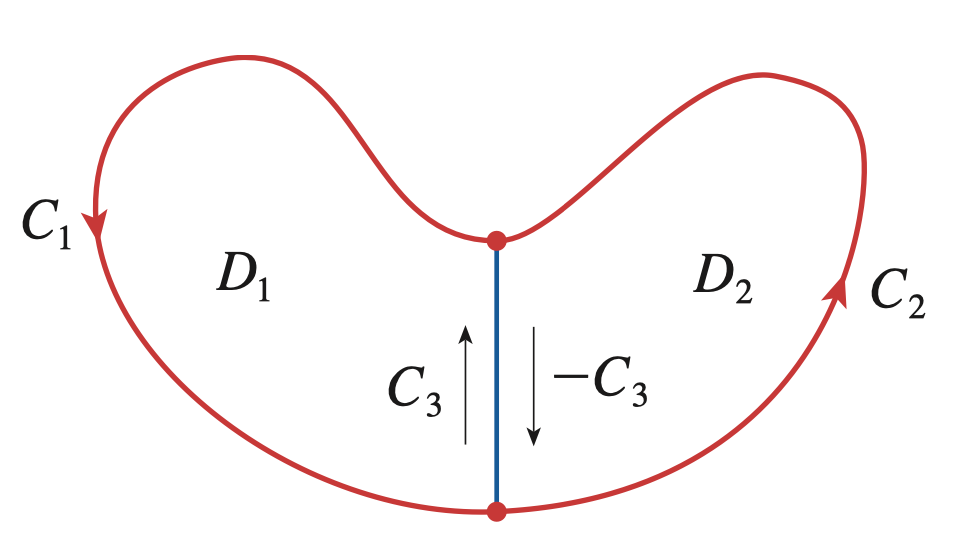
\includegraphics[scale=0.4]{FiniteUnion}
	\]
	\textbf{Green's theorem can be extended for regions which are finite unions of
	simple regions.}
	\[
		\oint_{C_1 \cup C_2}Pdx + Qdy = \iint\limits_{D} \pdv{Q}{x}-\pdv{P}{y}dA
	\]
	\subsection{16.5 Curl and Divergence}
	\begin{mybox}
		{Curl} If $\bm{F}= P \bm{i}+ Q \bm{j}+ R\bm{k}$ is a vector field on $\mathbb{R}
		^{3}$ and the partial derivatives of $P$, and $Q$ and $R$ all exist, then the
		curl of $F$ is the vector field defined by
		\[
			\textbf{curl }\bm{F}= \nabla \times \bm{F}=
			\begin{vmatrix}
				\vec{i}   & \vec{j}   & \vec{k}   \\
				\pdv{}{x} & \pdv{}{y} & \pdv{}{z} \\
				P         & Q         & R
			\end{vmatrix}
		\]
	\end{mybox}
	The curl of a conservative vector field, a vector field which is the gradient vector
	of a scalar function is the $\vec{0}$ Therefore, if the curl of a vector field
	is not the $0$ vector it is not conservative. If the curl is the $0$ vector,
	it is conservative if it is defined everywhere in $\mathbb{R}^{3}$.\\\\ The curl
	of a vector field can be a measure of rotation if the vector field models the velocities
	of a fluid. If $\bm{F}(x,y,z)=\vec{0}$ for some point $(x,y,z)$, then the fluid
	is irrotational at the point. The magnitude of the curl at that point is a
	measure of how fast the fluid moves around the axis.
	\begin{mybox}
		{Divergence} If $\bm{F}= P \bm{i}+ Q \bm{j}+ R\bm{k}$ is a vector field on $\mathbb{R}
		^{3}$ and the partial derivatives of $P$, and $Q$ and $R$ all exist, then the
		divergence of $F$ is the vector field defined by
		\[
			\textbf{div }\textbf{F}= \pdv{P}{x}+ \pdv{Q}{y}+ \pdv{R}{z}= \nabla \cdot \bm
			{F}
		\]
	\end{mybox}

	The divergence of curl $\bm{F}$ is div curl $\bm{F}= 0$. Notice also that the divergence
	of a vector field is a scalar field, whereas the curl of a vector field is a
	vector field. \\\\ If we think of a vector field $F$ as modeling a fluid field,
	then div $F$ models the tendency of the fluid to diverge from the point $(x,y,z
	)$.
	\[
		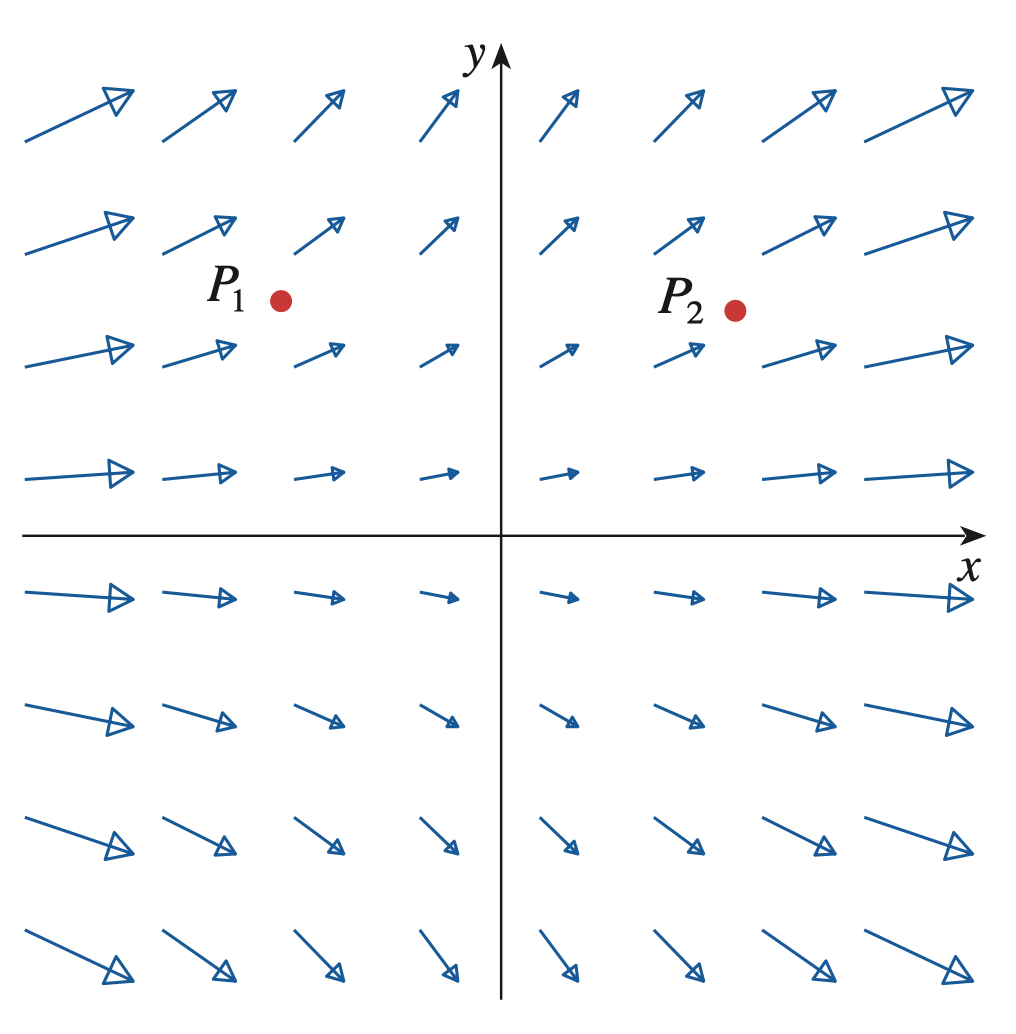
\includegraphics[scale=0.4]{Divergence}
	\]
	On this particular graph, for example, the divergence at point $P_{1}$ is
	negative because there is a net flow inwards as the arrows going out are
	smaller than those that are going in. The opposite is true for the other graph,
	where the divergence at $P_{2}$ is positive. With divergence and curl defined for
	vector fields, we can rewrite Green's theorem in their vector forms.
	\[
		\oint_{C} \bm{F}\cdot d\bm{r}= \iint\limits_{D} (\text{curl }\bm{F}) \cdot \bm
		{k}\,dA = \iint\limits_{D} \text{div}\,\bm{F}(x,y)\,dA
	\]

	\subsection{16.6 Parametric Surfaces and their areas}
	Similar to parametric curves in two dimensional space, we can parametrize a surface
	in three dimensional space using two variables. Particularly we can describe
	some surface $S$ by a vector function
	\[
		\bm{r}(u,v) = x(u,v) \bm{i}+ y(u,v) \bm{j}+ z(u,v) \bm{k}
	\]
	The set of all points $(x,y,z)$ such that
	\[
		x= x(u,v), y = y(u,v), z =z(u,v)
	\]
	marks the surface $S$
	\[
		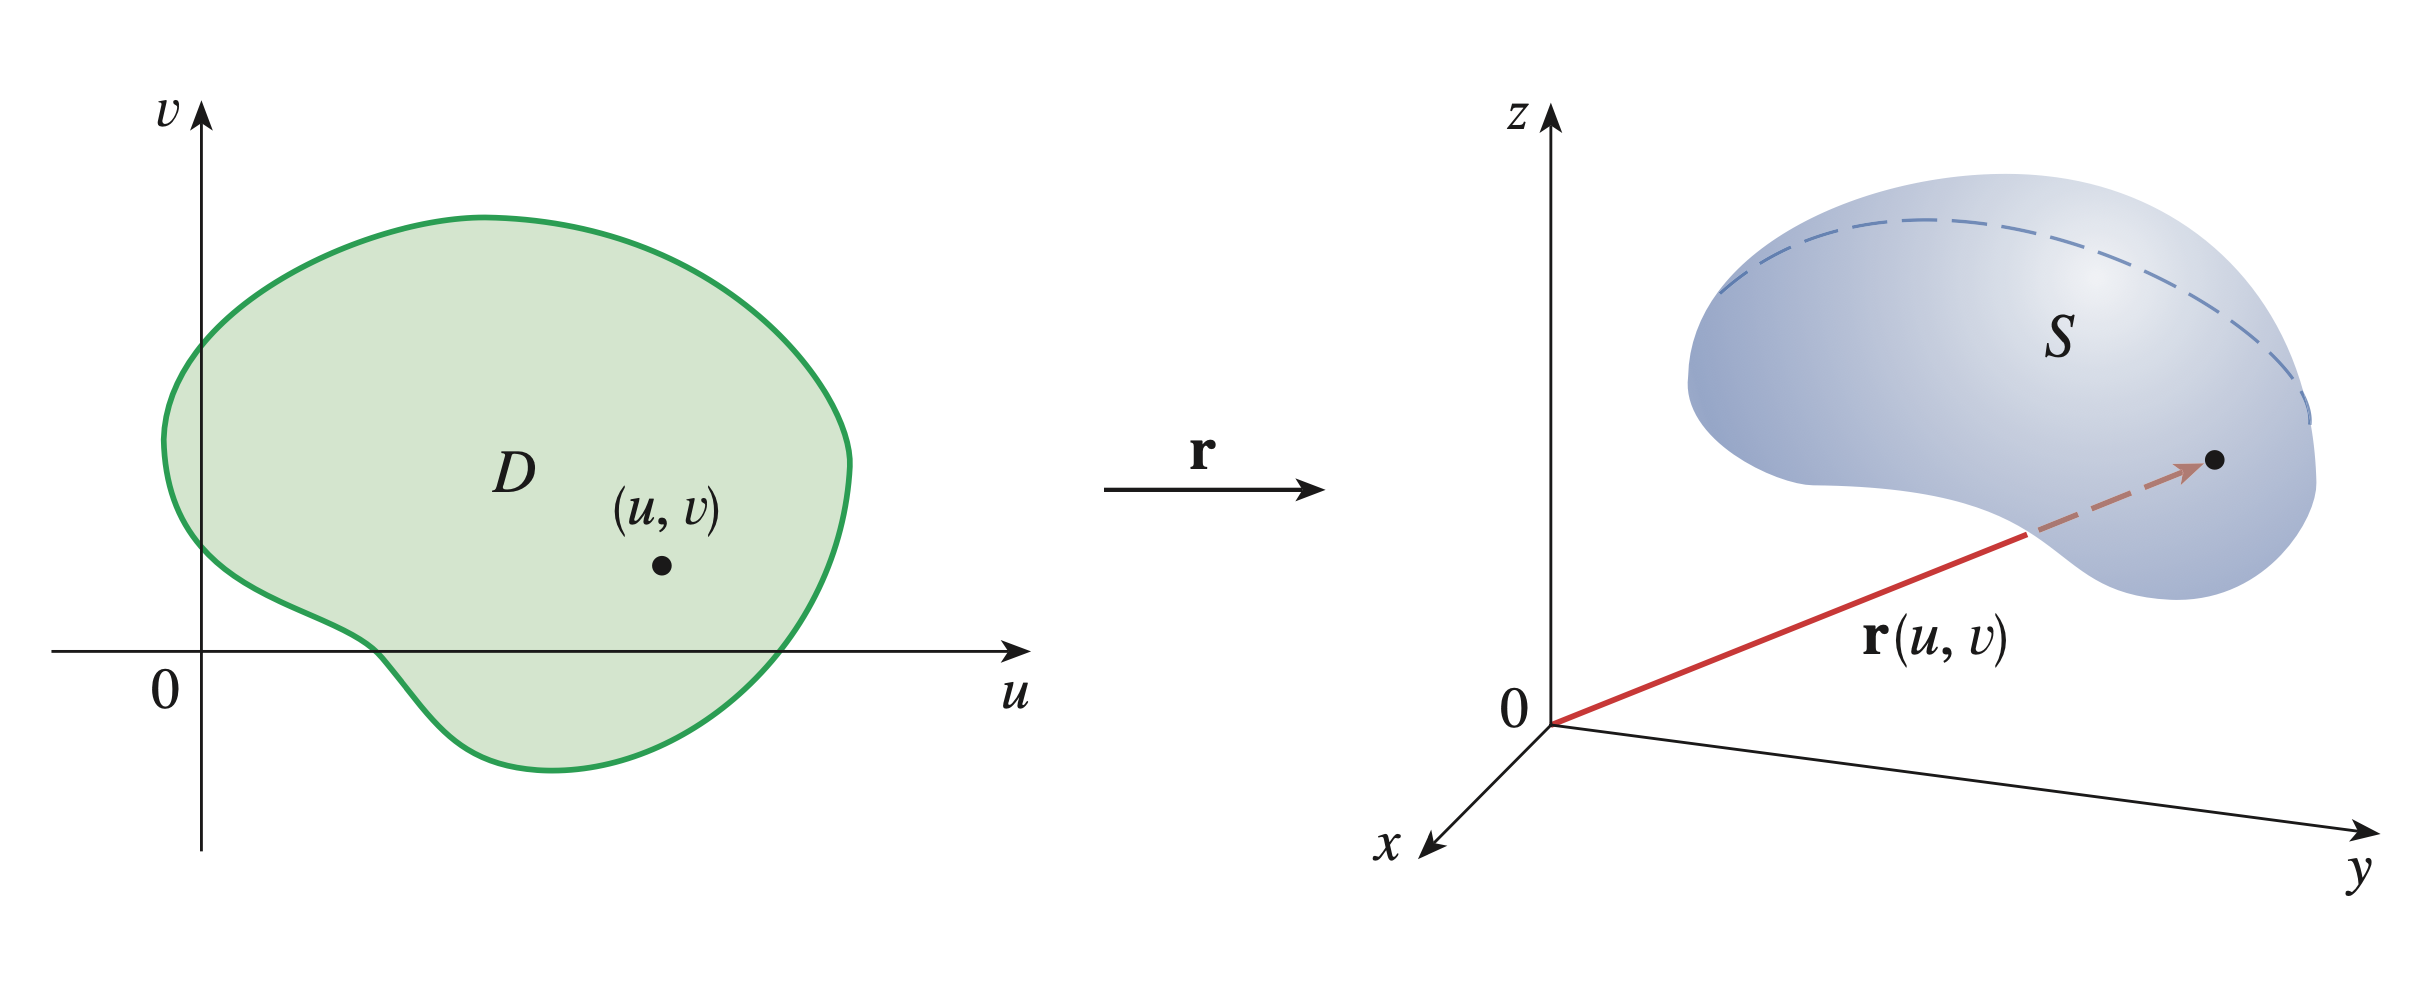
\includegraphics[scale=0.3]{ParametricSurfaces.png}
	\]
    If we fix on of the parameters of the function constant, what we obtain is a vector function of a single
    curve on the surface S
    \[
        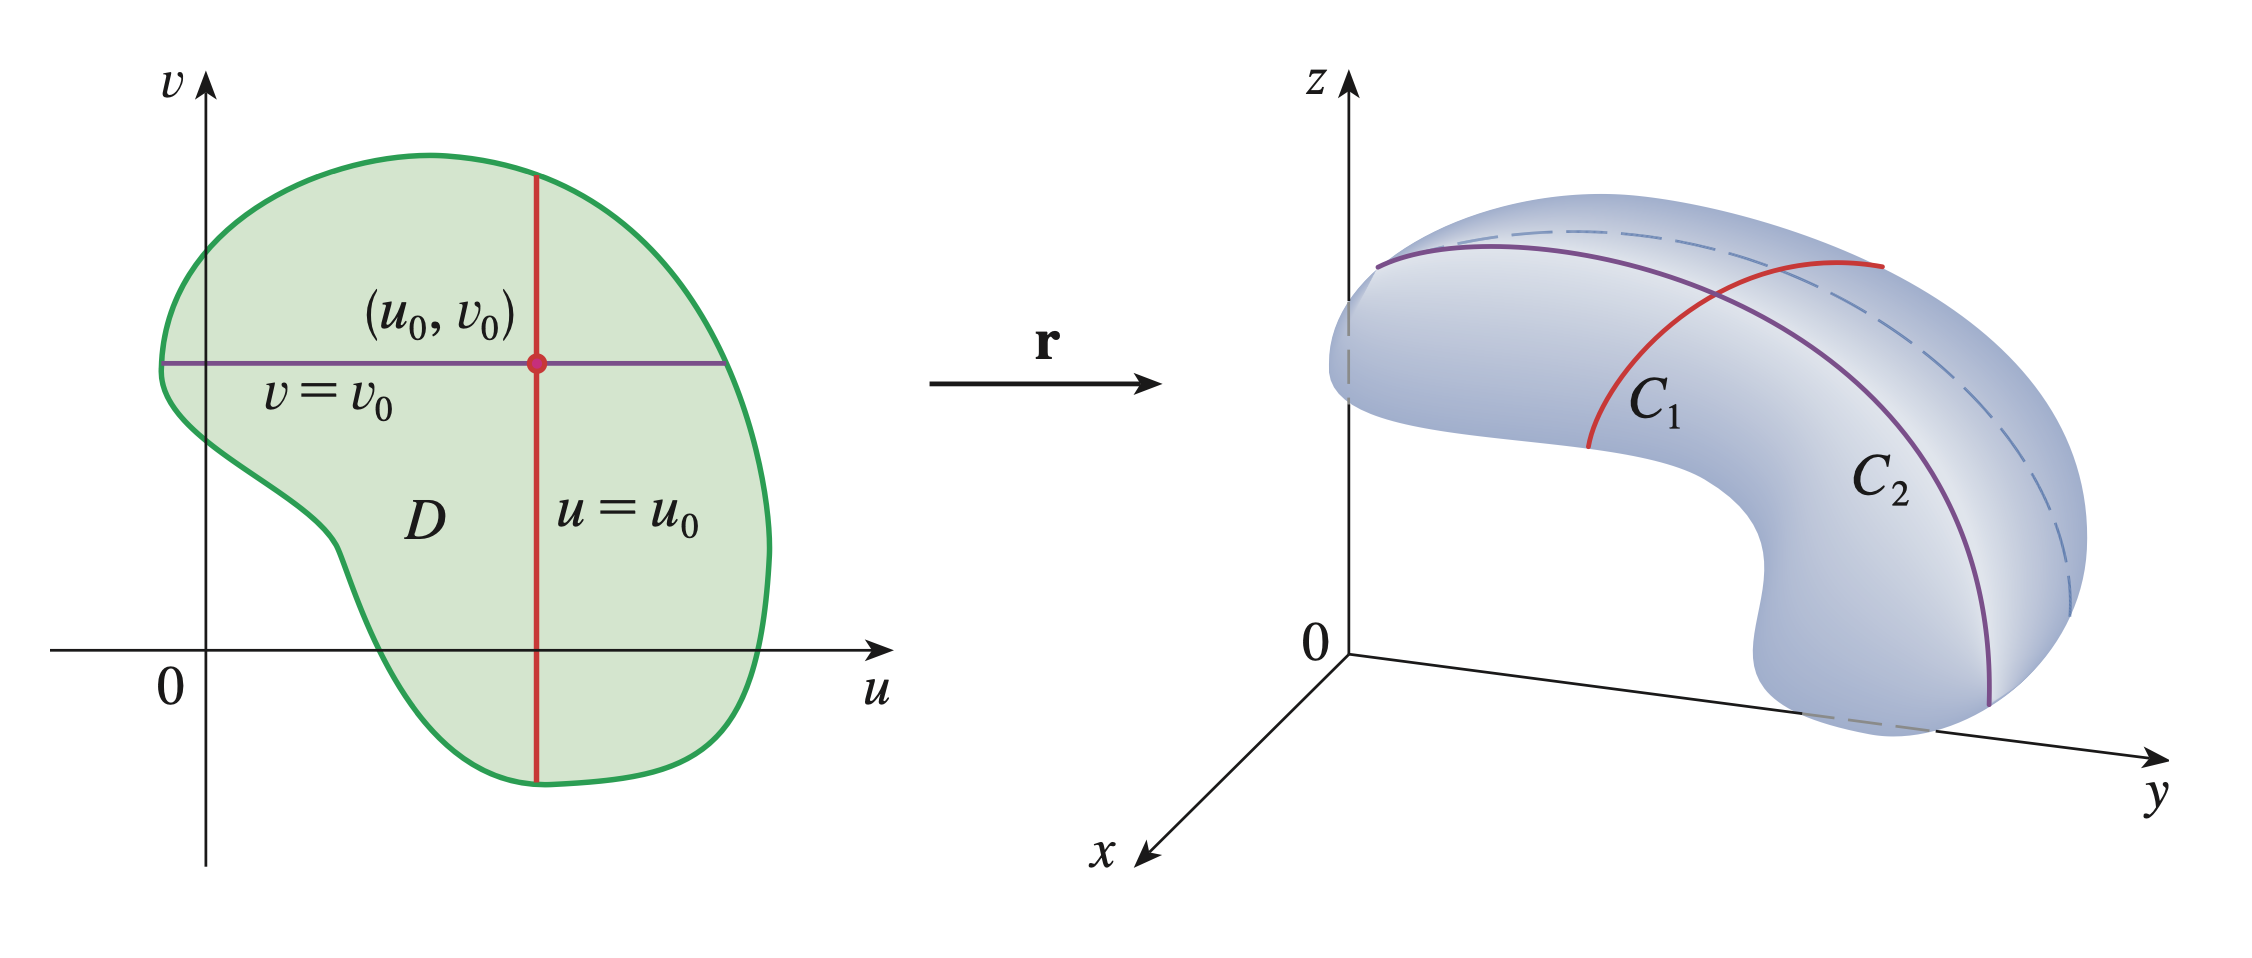
\includegraphics[scale=0.3]{ParametricCurvesOnSurface.png}
    \]
    Following a similar line of approach to that of finding the value of a function of two variables summed over a region
    it is possible to find the surface area of a parametric surface.
    \begin{mybox}{Surface area of a parametric surface}
    If a smooth parametric surface $S$ is given by the equation 
    \[
		\bm{r}(u,v) = x(u,v) \bm{i}+ y(u,v) \bm{j}+ z(u,v) \bm{k}
	\]
    ans $S$ is covered just once as $(u,v)$ ranges through the parameter domain then the surface area of $S$ is
    \[
		A(S) = \iint\limits_{D} \left| \bm{r}_u \times \bm{r}_v \right| dA
	\]
    \end{mybox}
    For some surface with equation $z =f(x,y)$ with $x=x$ and $y=y$ as its paramters.
    It is trivial to show that its surface area is equivalent to
    \[ 
    A(S) = \iint\limits_{D} \sqrt{1 + (\pdv{z}{x})^2 + (\pdv{z}{y})^2}
    \]
    \subsection{16.7 Surface Integrals}
    \begin{mybox}{Surface integral}
    It can be shown that the surface integral of $f$ also has an equivalent form of
    \[ \iint\limits_{S} f(x,y,z) dS = \iint\limits_{D}f(\bm{r}(u,v))\left|\bm{r}_u \times \bm{r}_v \right| dA\]
    \end{mybox}
    Any surface $S$ that can be defined by $x=x$, $y=y$ and $z=g(x,y)$ can be regarded as a parametric surface. It's possible to show
    that the surface integral of $f$ over $S$ is 
    \[ \iint\limits_{S} f(x,y,z) dS = \iint\limits_{D}f(x,y,g(x,y))\sqrt{\pdv{z}{x}^2+\pdv{z}{y}^2 + 1} dA \]
	\subsection{16.8 Stokes' Theorem}
	\begin{mybox}
		{Stokes' Theorem} Let $S$ be an oriented piecewise-smooth surface that is bounded
		by a simple, closed, piecewise-smooth boundary curve C with positive orientation.
		Let $\bm{F}$ be a vector field whose components have continuous partial
		derivatives on an open region in $\mathbb{R}^{3}$ that contains $S$. Then
		\[
			\int\limits_{C} \bm{F}\cdot d\bm{r}= \iint\limits_{S} \text{curl }\bm{F}\cdot
			d \bm{S}
		\]
	\end{mybox}
\end{document}
